\documentclass[10pt]{article}

\usepackage{amsmath}% http://ctan.org/pkg/amsmath
\usepackage{amsthm}
\usepackage{todonotes}
\usepackage[margin=1in]{geometry}
\usepackage{algorithm}
\usepackage{url}
\usepackage[noend]{algpseudocode}
\usepackage{mdframed}
\usepackage{tikz}
\usetikzlibrary{matrix,shapes,arrows,positioning,chains, calc}

%% defining new theorem environment for definition
\newtheorem{defn}{\textbf{Definition}}
\newtheorem{thm}{\textbf{Theorem}}
\newtheorem{cor}{\textbf{Corollary}}
\newtheorem{lemma}{\textbf{Lemma}}

\renewcommand{\algorithmicrequire}{\textbf{Input:}}
\renewcommand{\algorithmicensure}{\textbf{Output:}}

\begin{document}
\title{{\sf AND\=aNA-v2}: Application-Layer Support for \\ Low-Latency Bidirectional Anonymous Traffic in NDN \\ \emph{Design Specification Document}}
\author{Christopher A. Wood \\ UC Irvine \\ {\tt woodc1@uci.edu}}
\date{\today}
%\thanks{TODO}
\maketitle

%%% ABSTRACT
\begin{abstract}
This report documents the motivation, design, and implementation plan for the new version of {\sf AND\=aNA} to support highly efficient bidrectional traffic with low-latency in NDN. Weeks 1-3 of this project were spent setting up the experimental testbed and ramping up with the {\sf AND\=aNA} design and source code; weeks 4-6 were spent designing and running experiments to gather performance data for {\sf AND\=aNA}; weeks 7-8 were spent on the design of {\sf AND\=aNA-v2} and preliminary attempts at its implementation; weeks 9-10 were spent finalizing the design, completing the implementation, and gathering experimental data that can be used to compare against {\sf AND\=aNA}.
\end{abstract}

%%%%%%%%%%%%%%%%%%%%%
%%% MAIN CONTENT
%%%%%%%%%%%%%%%%%%%%%

\section{Overview} \label{sec:overview}
With the possibile adoption of NDN or any flavor of information-centric networking as the future Internet architecture in the near future, support for low-latency, bidirectional traffic may prove very useful for a variety of use cases. Consider the scenario in which two parties wish to exchange voice or video content over NDN, such as the case with Skype and related applications. Jacobson et al. \cite{voccn} have already studied the efficiencies of such content-heavy and QoS-strict applications over CCN. Unfortunately, support for such applications becomes much more difficult when one, or both, of the parties wishes to remain anonymous. Such is the case in settings where voice or video content is being streamed from \emph{some} person in a single organization, but the identity of said person needs to remain secret. A real-world instance where this may be useful is when such traffic needs to be exchanged between military organizations of unfriendly nations. Indeed, the identity of military personell participating in such voice or video conferences should remain secret for safety reasons. 

Application-layer support for anonymizing network traffic has already been implemented in the {\sf AND\=aNA} system \cite{andana}. However, in that work, the authors focus on a single, unidirectional client-producer scenario in which traffic latency, network jitter, and quality-of-service requirements were not specified nor mandated. In this work, we seek to amend the design of {\sf AND\=aNA} to support low-latency, bidrectional traffic applications with hard QoS and anonymity requirements. Consequently, this new design seeks to attain equivalent anonymity and privacy guarantees of {\sf AND\=aNA} while enjoying significantly higher performance - two factors that are often inversely related in practice. 

In the remainder of this document we discuss the motivation and details of our preliminary design for the new anonymizing application, dubbed {\sf AND\=aNA-v2}, as well as our implementation strategy. In order to avoid confusion and repetition throughout the rest of the document, all common terminology used throughout is specified and clarified in Table \ref{tab:notation}. Also, for simplicity, we denote the global system security parameter as $\kappa$, unless otherwise specified. 

\begin{table}
\centering
\caption{Notation used in the presentation of this work.}
\label{tab:notation}
  \begin{tabular}{| r | l |} \hline
  $\mathsf{C}$ & Set of all consumers  \\
  $\mathsf{P}$ & Set of all producers  \\ 
  $\mathsf{R}$ & Set of all routers  \\
  $\mathsf{IF}$ & Set of all interfaces on all routers  \\
  $\mathsf{if}_i^r \in \mathsf{IF}$ & Interface $i$ of router $r$  \\
  $(pk_i, sk_i)$ & Public/private key pair for router $r$  \\
  $\overline{\mathsf{int}}_{i}^{j}$ & Encrypted interest wrapped from router $i$ to router $j$ ($i \leq j$)  \\
  $\mathcal{A}$ & Adversary \\ 
  $u$ & Entity in the network (consumer or producer) \\
  $u \to_{\mathsf{int}} r$ & Entity $u$ sends interest to router $r$  \\ 
  $\mathsf{int} \to \mathsf{if}_i^r$ & Interest $\mathsf{int}$ is sent to interface $i$ of router $r$ \\
  $r \in \mathsf{R}$ & An anonymizing router (AR) \\ 
  $\mathcal{E}_{pk_i}(\cdot)$ & Public key encryption using $pk_i$ \\ 
  $\mathcal{D}_{pk_i}(\cdot)$ & Public key decryption using $pk_i$ \\ 
  $\mathsf{Encrypt}_{k_i}(\cdot)$ & Symmetric key encryption using key $k_i$ \\ 
  $\mathsf{Decrypt}_{k_i}(\cdot)$ & Symmetric key decrypt using key $k_i$ \\ 
  $\mathsf{ST}$ & AR session table used to store session ID and digest tuples \\
  $\mathsf{PIT}$ & AR pending interest table \\
  $H$ & A collision resistant hash function on the domain $\{0,1\}^*$ to range $\{0,1\}^{\kappa}$ \\
  $F_k$ & A keyed pseudorandom function \\ 
  $\mathsf{Pad}$ & An arbitrary padding function that appends \emph{random} bits to a payload \\ \hline
  \end{tabular}
\end{table}

\section{Motivation}
The primary motivation for a new desgin of {\sf AND\=aNA} is to attain the same anonymity and privacy guarantees as {\sf AND\=aNA} with \emph{better} performance. The original design targeted a single use case in which performance, especially in the bidirectional setting, was not a primary concern. Indeed, there was both an asymmetric and symmetric (session-based) variant of {\sf AND\=aNA}, and while the latter enjoyed better speedups over the former it suffered the fatal flaw of not ensuring packet unlinkability. It is generally the case that unlinkability is merely sufficient for anonymity, rather than also being a necessary condition for anonymity. However, in the case of {\sf AND\=aNA}, packet linkability can lead to consumer and producer linkability, which immediately violates anonymity. For example, it is not difficult to hypothesize an adversary that eavesdrops on incoming and outgoing interests for a particular anonymous router, and who by doing so is able to determine that the incoming and outgoing session IDs are linked. In fact, a modified type of this kind of adversary was explicitly studied in the context of Tor by Murdoch and Danezis in \cite{tor-traffic-analysis}. In their work, the goal of the adversary in their ``linkability attack'' was to determine whether two separate data streams being served by two corrupted servers were initiated by the same consumer, and we suspect that such analysis could be augmented to work for {\sf AND\=aNA}. Specifically, repeating a packet linkability attack at each anonymous router in a circuit may therefore eventually lead to linkability between the producer and consumer. The use of application and environment contextual information has also been formally studied in \cite{attacking-unlinkability}, in which side channel and environment information (e.g., the deterministic behavior of an anonymous router always forwarding a packet upstead after unwrapping an interest received from some downstream router) is used to quantify the \emph{degree of unlinkability}. Furthermore, we remark that regardless of how such linkability information is acquired, it has been shown that it can lead to reduce consumer and producer anonymity beyond what is possible with general traffic analysis \cite{linkability-attacks}. 

As most of the literature focuses on mix-based anonymizing services like Tor, which inspired the original design of {\sf AND\=aNA}, it is clear that any form of linkability should be avoided in order to maintain consumer and producer anonymity. Therefore, the formal goal for {\sf AND\=aNA-v2} is to attain the same anonymity and privacy guarantees as the asymmetric variant of {\sf AND\=aNA}, which does not suffer from packet linkability issues, while simultaneously supporting high-throughput and low-latency traffic between two parties in a unidirectional or bidirectional circuit. In addition, we seek to design a more modular architecture that enables various levels of performance and security guarantees to be achieved based on the type of application traffic that is to be supported. 

At the heart of the {\sf AND\=aNA} is the notion of anonymizing routers and connection-oriented circuits, similar in spirit to the inner workings of TOR \cite{tor}. Anonymizing routers serve two purposes in {\sf AND\=aNA}: (1) to decapsulate and forward encrypted interests, along with content encryption keys, generated by a consumer until the cleartext interest arrives at the producer, and (2) to encapsulate sensitive content using the previously acquired encryption keys and relay the encrypted content downstream. In this way, the consumer generates an interest wrapped by several layers of encryption and receives a piece of content wrapped in several layers of encryption that it can easily decrypt. It is also important to note that since each anonymizing router operates at the application layer, it effectively serves as the producer for each downstream router in the {\sf AND\=aNA} circuit. Therefore, NDN policy dictates that such content \emph{must be signed}. Verification of content from upstream routers, however, is not mandatory. 

We also note that the current {\sf AND\=aNA} design has support for two types of circuits: asymmetric and symmetric session-based. In the asymmetric variant, all encrypted interests are done using a CCA-secure PKI scheme and all content is encrypted using a CCA-secure symmetric key encryption scheme. Conversely, in the session-based variant, all encrypted interests are protected using a CCA-secure symmetric key encryption scheme, where the key is identified using a unique session identifier sent in the cleartext along with the encrypted interests. This worsens anonymity because it provides a way to link packets to a single session (as previously discussed).

Putting together all of the design aspects of the current version of {\sf AND\=aNA}, we see that the following factors weigh in on the overall performance of the application:
\begin{enumerate}
  \item Content encryption
  \item Content signature generation
  \item Encrypted interest generation and anonymous router decryption
\end{enumerate} 
In {\sf AND\=aNA-v2} we seek to minimize the degree to which these factors affect interest and content encapsulation and decapsulation by integrating support for anonymous router \emph{state}, which is encapsulated in sessions, into anonymous circuits. The content of this state depends on the type of deployment that will be used by {\sf AND\=aNA-v2}. All possible deployments are described in detail in the following section.

% Sessions will exist for unidirectional traffic only, which therefore means that bidirection traffic, the ultimate focus of this work, will require two sessions to be established and maintained for the duration of the bidirectional application. This is done so that each party in the application need not use the same set of anonymous routers for communication. Not only does this free each consumer to select a random subset of anonymous routers $r_1,r_2,\dots,r_n$ from the set of total anonymous routers $\mathsf{R}$, but it may also help improve QoS guarantees by distributing the load of encapsulation and decapsulation among multiple nodes. Furthermore, sessions enable the establishment of long-term secrets that can be used to improve the efficiency of certain cryptographic operations, such as content encryption, signature generation, and signature verification. 

% TODO: need for more performance and better security (problems with ANDNAv1, what we can do better, why unlinkability is a bad thing - cite related work here)

\section{Modular Architecture and Configurations}
{\sf AND\=aNA-v2} offers a flexible design that can be tailored for the particular types of applications that require its anonymity services. There are four different dimensions along which {\sf AND\=aNA-v2} can be deployed, including (1) the type and techniques used for content signature generation and verification, (2) technique for establishing state in an anonymous router circuit, (3) decision whether or not to use regular router caches, and (4) circuit formation decision for bidirectional traffic. We describe each of the configuration parameters in detail below.

\begin{enumerate}
\item \textbf{Content signature generation and verification}
\begin{itemize}
  \item Full reliance on PKI signatures: In this mode, all content flowing downstream will be \emph{signed and verified} using the existing public and private key pairs from the existing PKI-infrastructure. 

  \item Per-hop MAC and PKI-based signatures for NDN: In this mode, the last anonymous router in an anonymous circuit (i.e., the router closest to the producer) will verify the initial piece of content using the public key of the producer, and, upon success, will MAC the newly encrypted content to be sent downstream. This router will also digitally sign the encrypted content and MAC tag using its private key so as to conform to the original NDN specification \cite{ndn-tech-report}. All subsequent downstream routers will strip the NDN-layer signature from the upstream router, verify the MAC using a shared symmetric key, re-MAC their newly encrypted content, and again digitally sign the result before sending the entire collection downstream. \footnote{While the MAC may be perceived as redundant since the encrypted content is already digitally signed, observe that MAC generation and verification is significantly more efficient than a single public key signature verification. Therefore, by only incurring the public key signature verification overhead once at the last router and substituting it with MAC verification along all subsequent router hops, we still gain in efficiency.}

  \item Full reliance on router-to-router MACs: In the event that public-key digital signatures of each content sent downstream are not mandated, this technique will modify the above technique by removing the need for public-key signatures of encrypted content at each anonymous router in the circuit. In doing so, only the last router in the anonymous circuit will verify the initial plaintext content, and each reamining router will only rely on the per-hop MACs to ensure the authenticity of content as it flows downstream. Since the symmetric MAC keys are established by the consumer, such keys can be trusted. 
\end{itemize}

% \item[State initialization]
% \begin{itemize}
%   \item PKI-based transport: Using this technique, the consumer in an anonymous circuit will be responsible for generating and subsequently encrypting all state information that is to be stored and used by each router with their public key. Retrieval of this information is obtained by decrypting the interests and extracting the relevant session information which is inserted as a name component in the interest.
%   \item Diffie Hellman exchange: Using this technique, the consumer generates one half of the 
% \end{itemize}

\item \textbf{Circuit state establishment}
\begin{itemize}
  \item Pre-processing handshake: With the pre-processing handshake parameter configured, a consumer will perform the equivalent of a handshake with each anonymous router specified to partake in the anonymous circuit. This handshake procedure will not be used to acquire any meaningful data (i.e., encrypted interests are not sent in conjunction with interests to configure the anonymous router and state information). Once state is configured, each subsequent ``real'' interest issued during the lifetime of the circuit will be configured in such a way so that they all have the same length. This is done so that all interests are indistinguishable from the rest in the circuit.

  \item Piggyback circuit establishment: Without a pre-processing handshake procedure, anonymous circuit state is establishing by piggybacking the \emph{first} encrypted interest with all relevant session content. While this minimizes the overhead of the handshaking phase, it also imposes the requirement that all subsequent interests must again match the size of this first interest to ensure that interests are not distinguishable. 
\end{itemize}

\item \textbf{NDN cache utilization}
\begin{itemize}
  \item Caching enabled: With caching enabled, all anonymous routers through which anonymous interests traverse will persist the corresponding anonymous content in their caches. Since these routers do not possess any state information associated with the anonymous circuits they serve, any adversary who is able to compromise any subset of incoming and outgoing interfaces on one such router will not be able to use the anonymous interests or content flowing through the router to break producer or consumer anonymity. Therefore, caching in such routers only improves end-to-end latency for popular content (requested across the same circuit).

  \item Caching disabled: With caching disabled, no routers, including the {\sf AND\=aNA-v2} routers, will store content that is flowing downstream. This will not degrade anonymity or privacy in any way, but it may not benefit end-to-end latency since all encrypted interests will traverse along the entire length of the anonymous circuit. 
\end{itemize}

\item \textbf{Circuit formation}
\begin{itemize}
  \item Shared circuits for bidirectional communication: In this scheme, two parties participating in bidirectional communication will utilize the same circuit for all interests and content. In doing so, each router will also leverage the interest/content piggybacking technique presented in \cite{piggyback} to \emph{bundle} encrypted interests and decrypted content as they traverse the circuit between two parties. We expect the usage of these packets to benefit performance at the NDN layer by removing the need for FIB lookups and reducing the number of lower-layer invocations for retrieving and moving ``packets'' to and from router interfaces. 

  \item Independent circuits for bidirectional communication: In this configuration, parties $P_1$ and $P_2$ participating in bidirectional communication will independently generate circuits $r_1^1,\dots,r_n^1$ and $r_1^2,\dots,r_1^m$ of length $n$ and $m$, respectively, where $n$ need not equal $m$. In this mode it may be the case that there exists some $1 \leq 1 \leq n$ and $1 \leq j \leq m$ where $r_i^1 = r_j^2$, but since each party is oblivious to the circuit used by the other producer, this shared router does not adversely affect anonymity or privacy.
\end{itemize}

\end{enumerate}

In the following sections we describe the detailed design issues associated with each of these modes, but do so for the ``default'' configuration only. For example, we will describe the handshake-based circuit and session establishment procedure using the per-hop MAC and PKI-based signatures for NDN. We aim to present sufficient details so that replacing this content signature generation and verification configuration with, for example, full PKI-based signatures, the only difference is what information is included in the session state. It should be clear from context how the circuit and session handshake procedure would be modified in this instance.

   % * 3: type of content signature generation and verification
   %    * full PKI
   %    * per-hop MAC and NDN signatures
   %    * all NDN MAC (assume existence of offline key distribution protocol)
   % * 2: type of symmetric key establishment 
   %    * SSL/TLS or DH - forward secrecy or not 
   % * 2: handshake (current design) or non-handshake (interest packing)
   % * 2: cache or no cache content in intermediate routers
   %    * there is no consequence of caching content in routers since it's wrapped by encryption
   %    * there are also no anonymity problems either
   % * 2: separate (piggybacking) or independent circuits

\section{Handshake-Based Circuit and Session Establishment}
In this section we describe the procedure with which a circuit is established and used with a handshake procedure. Recall that our ultimate goal is to support highly efficient and anonymous bidirectional traffic. As such, the goals of the circuit and session establishment handshake using a list of $n$ anonymous routers $r_1,\dots,r_n$ are as follows:
\begin{enumerate}
\item Establish unique session IDs $\mathsf{session}_{i}$ and session IVs $\mathsf{SIV}_i$
\item Establish content encryption keys $E_{k_i}$ and initial counter values $\mathsf{EIV}_i$
\item Establish pairwise MAC keys $M_{k_i}$ used to sign and verify content
\end{enumerate}
The purpose of each of these session entities will become clear from the circuit initialization and usage procedures. After establishment, the circuit from the consumer $C$ to the producer $P$ should be similar to that shown in Figure \ref{fig:circuit}. We now describe the general protocol for establishing this type of session-based circuit from a consumer $C$ to a producer $P$ given $n$ anonymous routers. Recall that, in order to support bidirectional communication, $P$ would have to establish a similar circuit to $C$ with $m$ routers, where $m$ need not equal $n$. 

% \begin{algorithm}[ht!]
%   \caption{{\sf ServerRetrieveMACKey}}
%   \begin{algorithmic}[1]
%     \Require{$\mathsf{int}$}

%   % \State $(E_{k_n}, M_{k_n}, \mathsf{EIV}_n, \mathsf{session}_n, \mathsf{SIV}_n) \gets \overline{\mathcal{D}_{k}}(T)$
%   % \State \Return $(E_{k_n}, M_{k_n}, c_n, \mathsf{session}_n, \mathsf{IV}_n)$

%   \end{algorithmic}
% \end{algorithm}

\begin{algorithm}[ht!]
  \caption{{\sf ServerInterestHandler}}
  \begin{algorithmic}[1]
  \Require{Interest $\mathsf{int}$}
  % \State $k \gets \mathcal{D}_{sk_i}(\mathsf{int}[-1][0])$ // Recover session encryption key 
  \State $T := \mathsf{int}[-1]$
  \State $\mathsf{session}_i = T[0]$
  \If {$\mathsf{session}_i \in \mathsf{ST}$} \Comment{State initialized already, handle interest as usual}
    \State Handle the encrypted interest as needed...
    \State $\mathsf{SIV}_i = \mathsf{SIV}_i + 1$ (mod $2^{\kappa}$)
    \State $\mathsf{SIndex}_i := H(\mathsf{session}_i + \mathsf{SIV}_i)$
    \State Update $(\mathsf{SIndex}_i, \mathsf{session}_i, \mathsf{SIV}_i)$ in $\mathsf{ST}$
  \Else \Comment{Initialize the state}
    \State $k := \mathcal{D}_{sk_i}(T[1])$
    \State $(\mathsf{session}_i, E_{k_i}, M_{k_i}, M_{k_{i+1}} \mathsf{EIV}_i, \mathsf{SIV}_i, \mathsf{pad}) := \mathsf{Decrypt}_k(T[2:])$
    \State $\mathsf{SIndex}_i := H(\mathsf{session}_i + \mathsf{SIV}_i)$
    \State Persist $(\mathsf{session}_i, E_{k_i}, M_{k_i}, M_{k_{i+1}} \mathsf{EIV}_i, \mathsf{SIV}_i)$ to state 
    \State $\mathsf{resp} := \mathsf{Pad}(\mathsf{SIndex}_i)$ 
    \State $\mathsf{SIV}_i = \mathsf{SIV}_i + 1$ (mod $2^{\kappa}$)
    \State $\mathsf{SIndex}_i := H(\mathsf{session}_i + \mathsf{SIV}_i)$
    \State Update $(\mathsf{SIndex}_i, \mathsf{session}_i, \mathsf{SIV}_i)$ in $\mathsf{ST}$
    \State \Return $\mathsf{resp}$
  \EndIf

  % \If {$T[0] = \mathsf{SESSIONMAC}$}
  %   \State Parse the remaining tuple as $(M_{k}, \mathsf{session}_i, x)$
  %   \If{$\mathsf{session}_i$ not in state}
  %     \State \Return $\mathsf{Error}$
  %   \Else
  %     \State Persist $M_k$ as $M_{k_{i+1}}$ (the upstream MAC key) with session $\mathsf{session}_i$
  %     \State $x^* := \mathsf{MAC}_{M_{k}}(x)$
  %     \State $\mathsf{resp} := x^*$
  %     \State \Return $\mathsf{resp}$
  %   \EndIf
  % \Else
  %   \State $\mathsf{session}_i = T[0]$
    
  % \EndIf

  % $(\mathsf{session}_i, E_{k_i}, M_{k_i}, \mathsf{EIV}_i, \mathsf{SIV}_i)$

  % \State $(M_{k}, \mathsf{session}_i, x) := $ // Recover MAC key and randomness $x$
  % % \mathsf{SESSIONMAC}
  

  % \State $\mathsf{SIndex}_i := H(\mathsf{session}_i + \mathsf{SIV}_i)$
  % \State Persist $(\mathsf{session}_i, E_{k_i}, M_{k_i}, \mathsf{EIV}_i, \mathsf{SIV}_i)$ to state (override if already present)
  % \State $\mathsf{resp} := \mathsf{Pad}(\mathsf{SIndex}_i)$ 
  % \State $\mathsf{SIV}_i = \mathsf{SIV}_i + 1$ (mod $2^{\kappa}$)
  % \State $\mathsf{SIndex}_i := H(\mathsf{session}_i + \mathsf{SIV}_i)$
  % \State Update $(\mathsf{SIndex}_i, \mathsf{session}_i, \mathsf{SIV}_i)$ in $\mathsf{ST}$
  % \State \Return $\mathsf{resp}$

  \end{algorithmic}
\end{algorithm}

% \begin{algorithm}[ht!]
% \caption{{\sf ClientSendMACKey}}
%   \begin{algorithmic}[1]
%     \Require{$r_i$, $\mathsf{session}_i$, $M_{k}$}
%   \State $x \gets \{0,1\}^{\kappa}$
%   \State $x' := \mathsf{MAC}_{M_{k}}(x)$
%   \State $T \gets \mathsf{Pad}(\mathcal{E}_{pk_i}(\mathsf{SESSIONMAC}, M_{k}, \mathsf{session}_i, x))$
%   \State $\mathsf{int} := \mathsf{namespace}_i/\mathsf{int}$
%   \State $\mathsf{resp} := \mathsf{ccnget}(\mathsf{int})$ // reach out to the AR
%   \State $x^* := \mathsf{resp}[-1]$
%   \If{$x' \not= x^*$}
%     \State \Return $\mathsf{Fail}$
%   \Else
%     \State \Return $\mathsf{Pass}$
%   \EndIf

%   % \State $(E_{k_n}, M_{k_n}, \mathsf{EIV}_n, \mathsf{session}_n, \mathsf{SIV}_n) \gets \overline{\mathcal{D}_{k}}(T)$
%   % \State \Return $(E_{k_n}, M_{k_n}, c_n, \mathsf{session}_n, \mathsf{IV}_n)$

%   \end{algorithmic}
% \end{algorithm}

\begin{algorithm}[ht!]
\caption{{\sf ClientEstablishSession}}
  \begin{algorithmic}[1]
    \Require{$r_i$, $\mathsf{LastRouterFlag}$}
  \State $\overline{k} \gets \mathcal{E}_{pk_i}(k)$
  \State $T = ""$
  \If {$\mathsf{LastRouterFlag} = \mathsf{False}$}
    \State $T := (\mathsf{session}_i, E_{k_i}, M_{k_i}, M_{k_{i+1}} \mathsf{EIV}_i, \mathsf{SIV}_i)$
  \Else
    \State $T := (\mathsf{session}_i, E_{k_i}, M_{k_i}, \mathsf{Pad}(\epsilon), \mathsf{EIV}_i, \mathsf{SIV}_i)$
  \EndIf

  \State $T := \mathsf{Pad}(\overline{k} || \mathsf{Encrypt}_k(T))$

  \State $\mathsf{int} := \mathsf{namespace}_i/T$
  \State $\mathsf{resp} := \mathsf{ccnget}(\mathsf{int})$ // reach out to AR
  \If {$\mathsf{resp}[0] = \mathsf{SIndex}_i$} // Make sure the AR ACK'd correctly
    \State $\mathsf{SIV}_i = \mathsf{SIV}_i + 1$ (mod $2^{\kappa}$)
    \State $\mathsf{SIndex}_i := H(\mathsf{session}_i + \mathsf{SIV}_i)$
    \State Update $(\mathsf{SIndex}_i, \mathsf{session}_i, \mathsf{SIV}_i)$ in $\mathsf{ST}$
    \State \Return $\mathsf{Pass}$
  \Else
    \State \Return $\mathsf{Fail}$
  \EndIf
  % \State $(E_{k_n}, M_{k_n}, \mathsf{EIV}_n, \mathsf{session}_n, \mathsf{SIV}_n) \gets \mathsf{Decrypt}_{k}(\mathsf{resp})$
  % \State \Return $(E_{k_n}, M_{k_n}, c_n, \mathsf{session}_n, \mathsf{IV}_n)$

  \end{algorithmic}
\end{algorithm}

% \State $E_{k_i} \gets \{0,1\}^k$ for $k = 1,\dots,n$ // Encryption key
% \State $M_{k_i} \gets \{0,1\}^k$ for $k = 1,\dots,n$ // MAC key
% \State $c_i \gets \{0,1\}^k$ for $k = 1,\dots,n$     // counter IV
% \State $x \gets \{0,1\}^k$
% \State $\mathsf{session}_n := H(x)$
% \State $T' := (\mathsf{session}_n, E_{k_n}, c_n, M_{k_n})$
% \State $T_n := \mathcal{E}_{pk_n}(T')$


\begin{algorithm}[ht!]
\caption{{\sf EstablishCircuit}}
  \begin{algorithmic}[1]
    \Require{Anonymous routers $r_1,r_2,\dots,r_n$ ($n \geq 2$) with public keys $pk_1,pk_2,\dots,pk_n$.}

\For {$i = 1$ \textbf{ to } $n$}
  \State $k \gets \{0,1\}^{\kappa}$
  \State $E_{k_i} \gets \{0,1\}^{\kappa}$ // Encryption key
  \State $M_{k_i} \gets \{0,1\}^{\kappa}$ // MAC key
  \State $\mathsf{EIV}_i \gets \{0,1\}^{\kappa}$     // counter IV
  \State $x \gets \{0,1\}^{\kappa}$
  \State $\mathsf{SIV}_i \gets \{0,1\}^{\kappa}$ // session IV
  \State $\mathsf{session}_i := H(x)$ // session ID
  \State $\mathsf{SIndex}_i := H(\mathsf{session}_i + \mathsf{SIV}_i)$
  \State Persist $(\mathsf{session}_i, E_{k_i}, M_{k_i}, \mathsf{EIV}_i, \mathsf{SIV}_i)$ to state and store $(\mathsf{SIndex}_i, \mathsf{session}_i, \mathsf{SIV}_i)$ in $\mathsf{ST}$
\EndFor
% \State $(E_{k_n}, M_{k_n}, c_n, \mathsf{session}_n, \mathsf{IV}_n) := \mathsf{ClientEstablishSession}(r_n)$
\For{$i = 1$ \textbf{ to } $n$}
  \If {$i = n$}
    \If {$\mathsf{ClientEstablishSession}(r_n, \mathsf{True}) = \mathsf{Fail}$}
      \State \Return $\mathsf{Fail}$
    \EndIf
  \Else
    \If {$\mathsf{ClientEstablishSession}(r_n, \mathsf{False}) = \mathsf{Fail}$}
      \State \Return $\mathsf{Fail}$
    \EndIf
  \EndIf
  % \If{$\mathsf{ClientSendMACKey}(r_i, \mathsf{session}_i, M_{k_{i+1}}) = \mathsf{Fail}$}
  %   \State \Return $\mathsf{Fail}$
  % \EndIf
  % \State $\mathsf{session}_{i} := H(\mathsf{session}_n \bigoplus_{j=i}^{n} E_{k_j})$
  % \State $T' := (\mathsf{session}_i, E_{k_i}, c_i, M_{k_i}, M_{k_{i+1}})$
  % \State $T_n := \mathcal{E}_{pk_i}(T_i)$
  % \State $\mathsf{EstablishSession}(T_i)$
\EndFor
  \end{algorithmic}
\end{algorithm}

Notice that by this procedure, no two routers will share the same session identifier even though they partake in the same circuit since they generate session identifiers independent and uniformly at random from $\{0,1\}^{\kappa}$. Also, the {\sf ServerEstablishSession} and {\sf ServerRetrieveMACKey} procedures are asynchronous and only invoked in response to the respective interest.

\begin{figure}[ht!]
\begin{center}
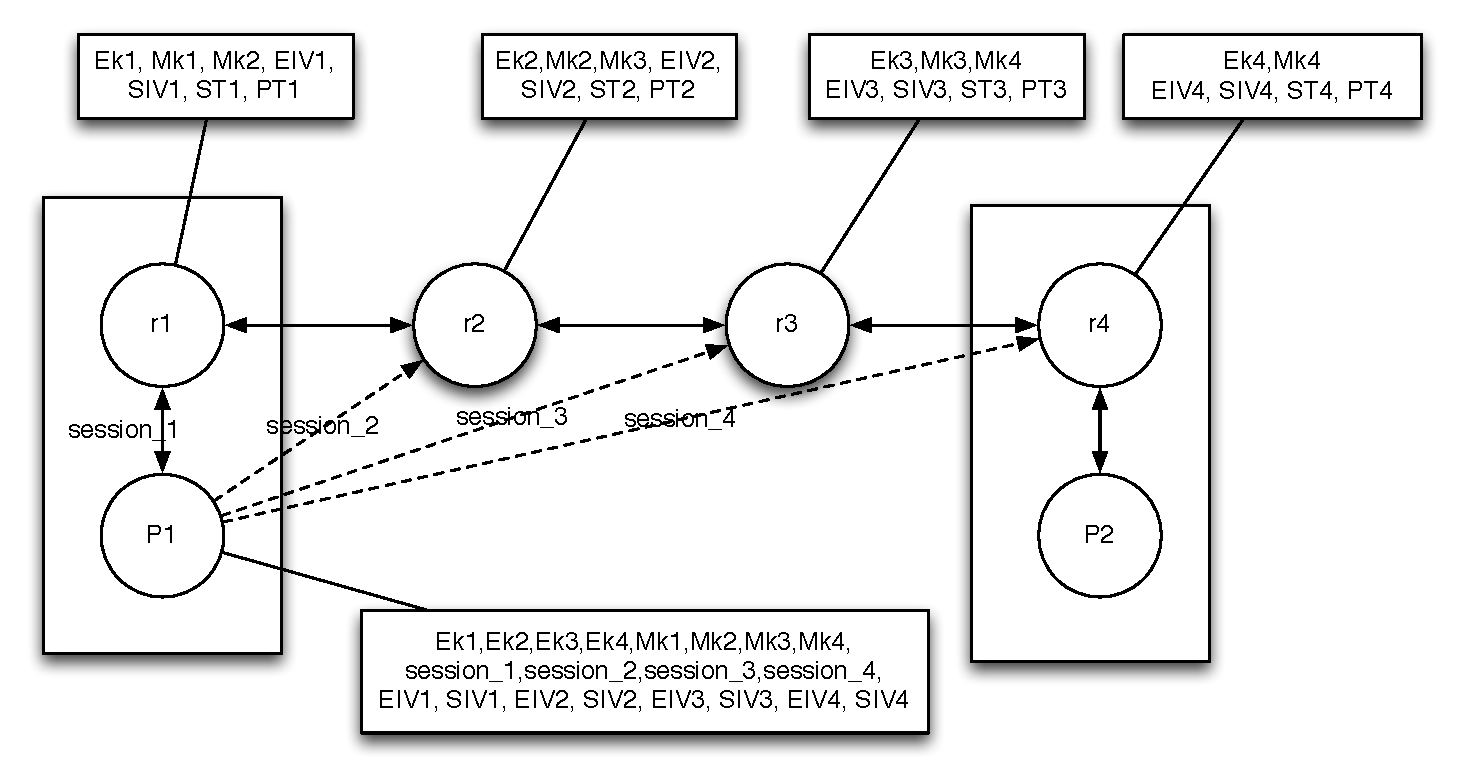
\includegraphics[scale=0.5]{./images/circuit.pdf}
\end{center}
\caption{Sample session-based circuit between a consumer $C$ and producer $P$ with ARs $r_1,r_2,r_3,r_4$, where the end routers on the path are run on the same node as $C$ and $P$.}
\label{fig:circuit}
\end{figure}

\subsection{Circuit Usage}
% We note that anonymous routers must be chosen in a \emph{mutually excluse} manner, meaning that they do not change share the same name prefix or are from the same organization (see Figure \ref{fig:pool}). This requirement is needed for ensuring anonymity. 

After a circuit and the corresponding sessions have been created between the consumer and each anonymous router, usage of the circuit proceeds as per the original {\sf AND\=aNA} design. Specifically, there are three main operations that need to be defined: encrypted interest generation, AR interest forwarding, and AR content handling. In what we follows we present the details of each of these procedures as needed for {\sf AND\=aNA-v2}. We begin with the encrypted interest generation procedure (shown in Algorithm \ref{alg:enc_int_gen}) in which a consumer $C$ particpating in a particular \emph{application} session with a producer $P$ wraps an interest for the session to be sent into the anonymizing circuit. A wrapped (encrypted) interest from $r_i$ to $r_j$ ($i \leq j$) is denoted as $\overline{\mathsf{int}}_i^j$, meaning that the original plaintext interests $\mathsf{int}$ cannot be retrieve unless encrypted by each router $r_i,r_{i+1},\dots,r_j$, in that order. Thus, the original wrapped interest is denoted as $\overline{\mathsf{int}}_1^n$.

\begin{figure}[ht!]
\begin{center}
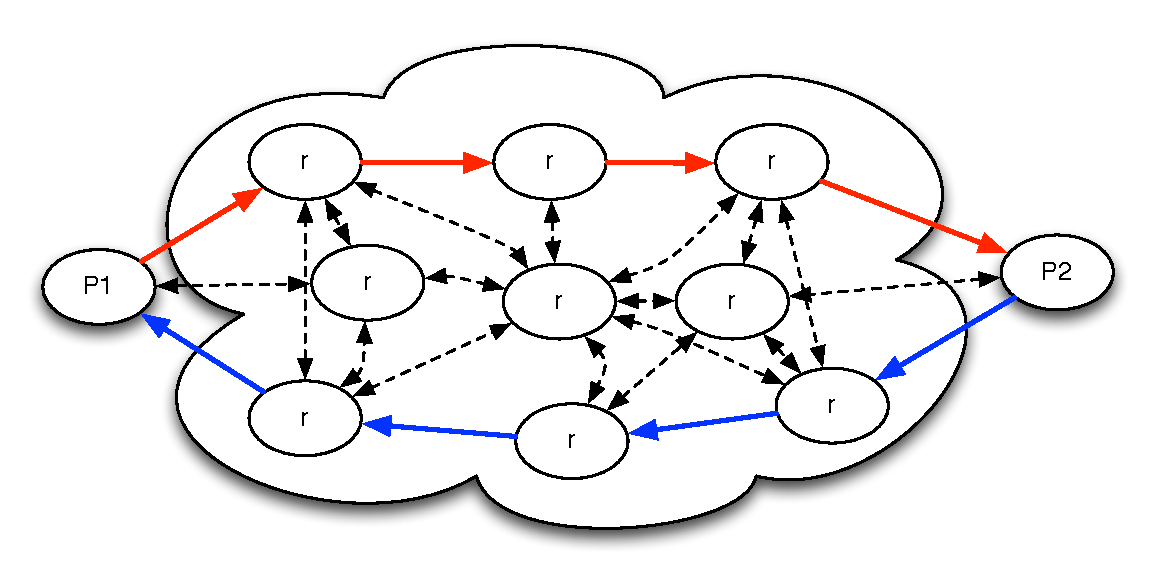
\includegraphics[scale=0.5]{./images/pool.pdf}
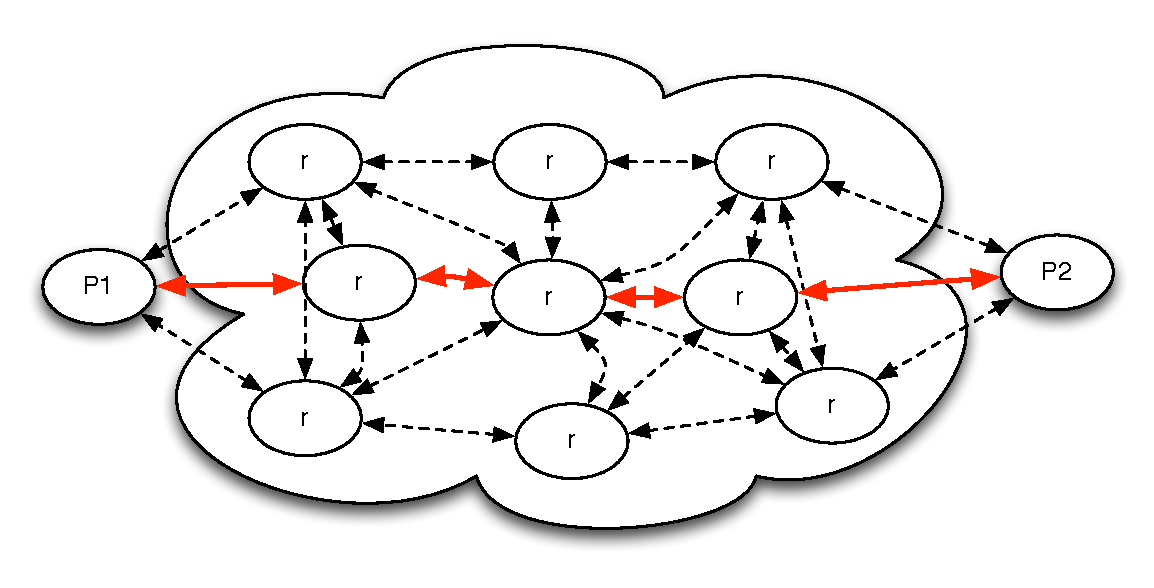
\includegraphics[scale=0.5]{./images/pool_same.pdf}
\end{center}
\caption{The first image depicts a sample bidirectional circuit configuration in which two parties communicate using mutually exclusive ARs in both directions. Note that it is not required for each circuit to be the same length, nor is it required that the intersection of the routers for each direction of the circuit to be empty (i.e., routers may \emph{unknowingly} support sessions traversing in both directions). The second image depicts the configuration where both parties knowingly share the same circuit.}
\label{fig:pool}
\end{figure}

\begin{algorithm}[ht!]
  \caption{Encrypted Interest Generation}
  \begin{algorithmic}[1]
    \Require{Interest $\mathsf{int}$, routers $r_1,r_2,\dots,r_n$ ($n \geq 2$) in circuit}
    \Ensure{Encrypted interest $\overline{\mathsf{int}}_{1}^{n}$}
\State $\overline{\mathsf{int}} = \mathsf{int}$
\For{$i = n$ \textbf{ downto } $1$}
  \State $\mathsf{SIndex}_i := H(\mathsf{session}_i + \mathsf{SIV}_i)$
  \State $\mathsf{SIV}_i = \mathsf{SIV}_i + 1$ (mod $2^{\kappa}$)
  \State $\overline{\mathsf{int}}_i^n = R_i / \mathsf{SIndex}_i / \mathsf{Pad}(\mathsf{Encrypt}_{E_{k_i}}(\overline{\mathsf{int}}, \mathsf{timestamp}))$
\EndFor
\State \Return $\overline{\mathsf{int}}_1^n$
\end{algorithmic}
\label{alg:enc_int_gen}
\end{algorithm}

\begin{algorithm}[ht!]
  \caption{AR Encrypted Interest Forwarding}
  \begin{algorithmic}[1]
    \Require{$\overline{\mathsf{int}}_i^j$}
    \Ensure{$(\overline{\mathsf{int}}_{i+1}^j, \mathsf{session}_i)$ or discarded packet}
\If{$\mathsf{SIndex}_i \in \mathsf{ST}_i$}
  \State Let $(\mathsf{session}_i, E_{k_i}, M_{k_i}, \mathsf{EIV}_i, \mathsf{SIV}_i)$ be the session information associated with $\mathsf{SIndex}_i$
  \State $\mathsf{SIV}_i := \mathsf{SIV}_i + 1$ (mod $2^{\kappa}$)
  \State $\mathsf{SIndex}_i := H(\mathsf{session}_i + \mathsf{SIV}_i)$
  \State Update $(\mathsf{SIndex}_i, \mathsf{session}_i, \mathsf{SIV}_i)$ in the session table $\mathsf{ST}_i$
  \State $(\overline{\mathsf{int}}_{i+1}^{j}, timestamp) := \mathsf{Decrypt}_{E_{k_i}}(\overline{\mathsf{int}}_{i}^{j})$
  \If{decryption fails or $\mathsf{timestamp}$ is not current}
    \State Discard $\overline{\mathsf{int}}_{i}^{j}$
  \Else
    \State Persist tuple $T_i = (\overline{\mathsf{int}}_{i}^{j}, \overline{\mathsf{int}}_{i+1}^{j}, \mathsf{session}_i)$ to pending interest table $\mathsf{PIT}_i$
    \State \Return $(\overline{\mathsf{int}}_{i+1}^{j}, \mathsf{session}_i)$
  \EndIf
\Else
  \State Discard $\overline{\mathsf{int}}_{i}^{j}$ \Comment{Some form of interest flooding prevention should be employed here}
\EndIf
\end{algorithmic}
\label{alg:enc_int_forward}
\end{algorithm}

\begin{algorithm}[ht!]
  \caption{AR Content Handling}
  \begin{algorithmic}[1]
    \Require{Content $\overline{data_{i+1}^j}$ in response to interest $\overline{\mathsf{int}}_{i+1}^{j}$}
    \Ensure{Encrypted data packet $data_{i}^j$}
\State Recover tuple $T_i = (\overline{\mathsf{int}}_{i}^{j}, \overline{\mathsf{int}}_{i+1}^{j}, \mathsf{session}_i)$ based on $data_{i+1}^j$
\State Parse $\overline{data_{i+1}^j}$ as a tuple $(data_{i+1}^j, \sigma_{i+1}, \sigma_p)$
\If{$\sigma_{i+1} = \epsilon$ and $M_{k_{i+1}} = \epsilon$} 
  \State Let $pk_p$ be the public key associated with the producer
  \If{$\sigma_p = \mathsf{Verify}_{pk_{p}}(data_{i+1}^j)$}
    \State Pass
  \Else
    \State \Return $\mathsf{Error}$ \Comment{Producer signature verification did not pass}
  \EndIf
\ElsIf{$\sigma_{i+1} \not= \epsilon$ and $M_{k_{i+1}} \not= \epsilon$}
  \If{$\sigma_{i+1} = \mathsf{Verify}_{M_{k_{i+1}}}(data_{i+1}^j)$}
    \State Pass
  \Else
    \State \Return $\mathsf{Error}$ \Comment{MAC verification did not pass}
  \EndIf
\Else \Comment{There was either a tag or we don't have the upstream MAC key - either way, we error}
  \State \Return $\mathsf{Error}$
\EndIf

\State Remove signature $\sigma_p$ and name from $data_{i+1}^j$ %\Comment{This signature may have come from the producer or an AR}
\State Create new empty data packet $data_i^j$
\State Set name on $data_i^j$ as the name on $\overline{\mathsf{int}}_{i}^{j}$
\State $data_i^j := \mathsf{Encrypt}_{E_{k_i}}(data_i^j)$
\State $\sigma_i := \mathsf{MAC}(data_i^j)$
\State $\overline{data_{i}^j} = (data_i^j, \sigma_i)$
\State \Return $\overline{data_{i}^j}$ \Comment{Digital signature applied before sending downstream}

\end{algorithmic}
\label{alg:ar_content_handler}
\end{algorithm}

\begin{figure}[ht!]
\begin{center}
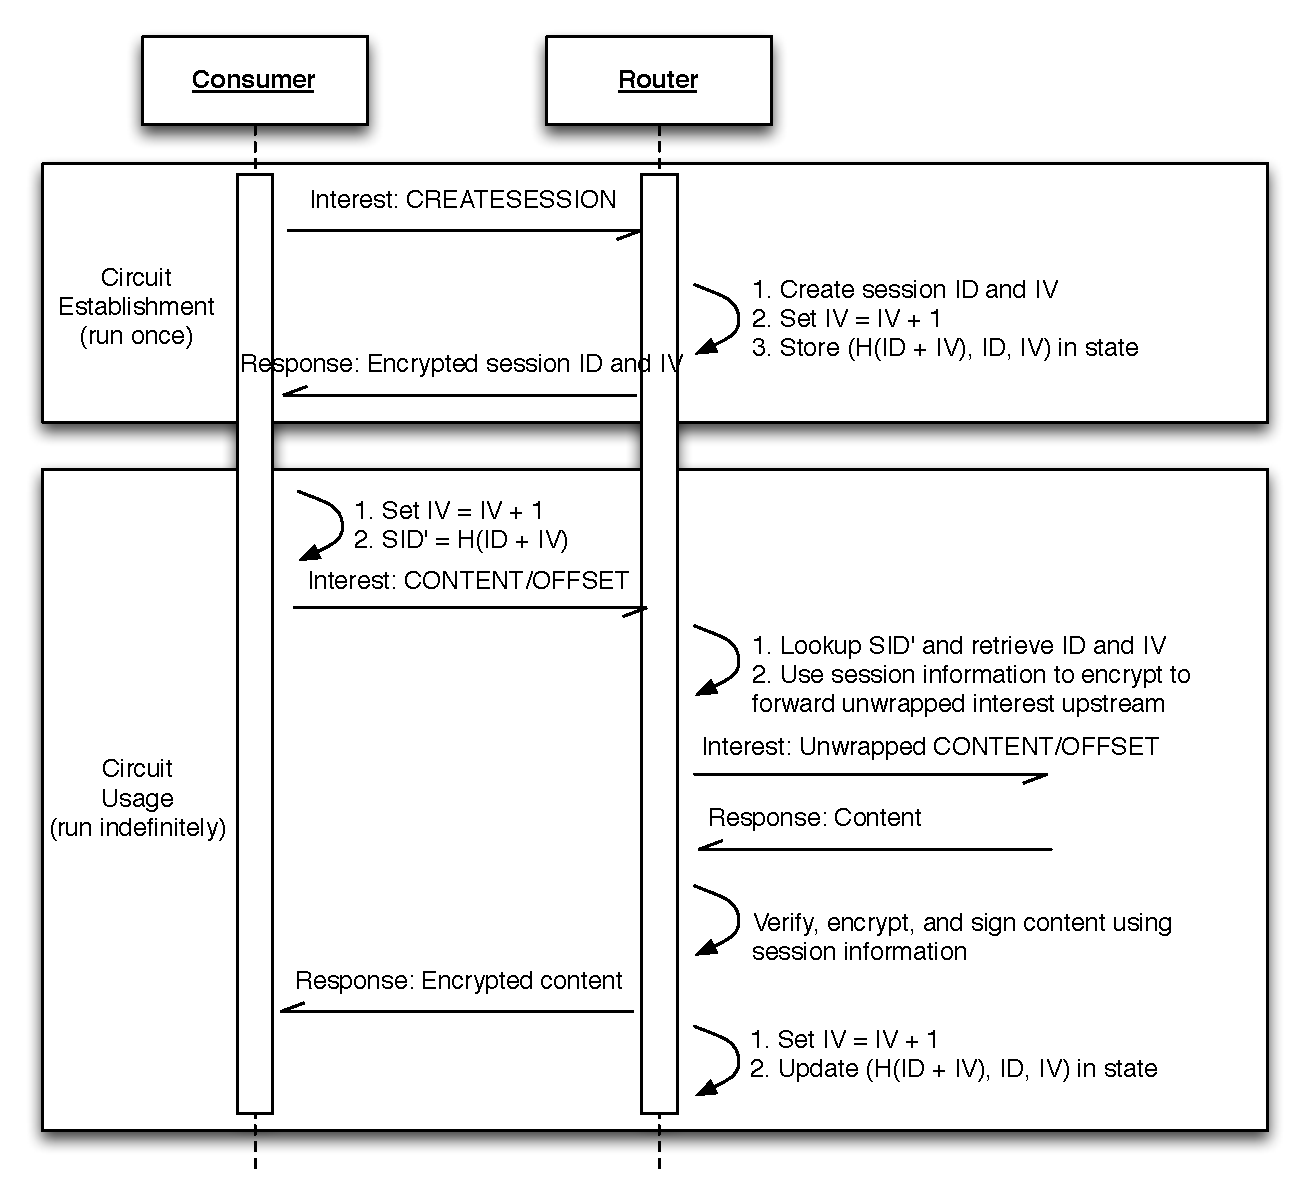
\includegraphics[scale=0.65]{./images/circuit_usage.pdf}
\end{center}
\caption{Visual depiction of the interaction between the consumer and the first hop router. The procedure repeats in the same manner for all further upstream routers after each interest is unrolled and resulting content is encrypted.}
\label{fig:circuit_usage}
\end{figure}

\section{Piggybacked Circuit and Session Establishment}
In this section we describe the details of the piggybacked circuit establishment technique. For simplicity, we will assume the same session information as in the handshake variant of circuit and session establishment. Details about how to attain uniform packet size is omitted until Section \ref{sec:details}. The following algorithms describe the piggybacking session establishment approach. Observe that the only real distinction between this and the handshaking procedure is that the circuit establishment logic is now embedded in each algorithm (i.e., the consumer and routers must differentiate the interest between a new session creation interest and one that simply corresponds to a normal encrypted interest). In particular, the content encapsulation procedure is no different from the handshake-based circuit establishment method.

\begin{algorithm}[ht!]
  \caption{Encrypted Interest Generation}
  \begin{algorithmic}[1]
    \Require{Interest $\mathsf{int}$, circuit length $n$, AR pool $\mathcal{R}$, global boolean $\mathsf{SessionCreated}$}
    \Ensure{Encrypted interest $\overline{\mathsf{int}}_{1}^{n}$}

\If{$\mathsf{SessionCreated} = \mathsf{True}$}
  \State $\overline{\mathsf{int}} = \mathsf{int}$
  \For{$i = n$ \textbf{ downto } $1$}
    \State $\mathsf{SIndex}_i := H(\mathsf{session}_i + \mathsf{SIV}_i)$
    \State $\mathsf{SIV}_i = \mathsf{SIV}_i + 1$ (mod $2^{\kappa}$)
    \State $\overline{\mathsf{int}}_i^n = R_i / \mathsf{Pad}(\mathsf{SIndex}_i || \mathsf{Encrypt}_{E_{k_i}}(\overline{\mathsf{int}}, \mathsf{timestamp}))$
  \EndFor
  \State \Return $\overline{\mathsf{int}}_1^n$
\Else

\For {$i = 1$ \textbf{ to } $n$} \Comment{Initialize state}
  \State $k \gets \{0,1\}^{\kappa}$
  \State $E_{k_i} \gets \{0,1\}^{\kappa}$ // Encryption key
  \State $M_{k_i} \gets \{0,1\}^{\kappa}$ // MAC key
  \State $\mathsf{EIV}_i \gets \{0,1\}^{\kappa}$     // counter IV
  \State $x \gets \{0,1\}^{\kappa}$
  \State $\mathsf{SIV}_i \gets \{0,1\}^{\kappa}$ // session IV
  \State $\mathsf{session}_i := H(x)$ // session ID
  \State $\mathsf{SIndex}_i := H(\mathsf{session}_i + \mathsf{SIV}_i)$
  \State Persist $(\mathsf{session}_i, E_{k_i}, M_{k_i}, \mathsf{EIV}_i, \mathsf{SIV}_i)$ to state and store $(\mathsf{SIndex}_i, \mathsf{session}_i, \mathsf{SIV}_i)$ in $\mathsf{ST}$
\EndFor
\State $\overline{\mathsf{int}} = \mathsf{int}$
\For{$i = n$ \textbf{ downto } $1$} \Comment{Wrap the state up with the interest}
  \State $k \gets \{0,1\}^{\kappa}$
  \State $\overline{k} \gets \mathcal{E}_{pk_i}(k)$
  \State $T = ""$

  \If {$i = n$}
    \State $T := (\mathsf{session}_i, E_{k_i}, M_{k_i}, M_{k_{i+1}} \mathsf{EIV}_i, \mathsf{SIV}_i)$
  \Else
    \State $T := (\mathsf{session}_i, E_{k_i}, M_{k_i}, 0^{\kappa}, \mathsf{EIV}_i, \mathsf{SIV}_i)$
  \EndIf

  \State $T := \mathsf{Pad}(\overline{k} || \mathsf{Encrypt}_k(T) || \mathsf{Encrypt}_{E_{k_i}}(\overline{int}, timestamp))$
  \State $\mathsf{SIndex}_i := H(\mathsf{session}_i + \mathsf{SIV}_i)$
  \State $\mathsf{SIV}_i = \mathsf{SIV}_i + 1$ (mod $2^{\kappa}$)
  \State $\overline{\mathsf{int}}_i^n = R_i / \mathsf{Pad}(\mathsf{SIndex}_i || \mathsf{Encrypt}_{E_{k_i}}(\overline{\mathsf{int}}, \mathsf{timestamp}))$
\EndFor
\State \Return $\overline{\mathsf{int}}_1^n$  
  
  % \State $E_{k_i} \gets \{0,1\}^{\kappa}$ // Encryption key
  % \State $M_{k_i} \gets \{0,1\}^{\kappa}$ // MAC key
  % \State $\mathsf{EIV}_i \gets \{0,1\}^{\kappa}$     // counter IV
  % \State $x \gets \{0,1\}^{\kappa}$
  % \State $\mathsf{SIV}_i \gets \{0,1\}^{\kappa}$ // session IV
  % \State $\mathsf{session}_i := H(x)$ // session ID
  % \State $\mathsf{SIndex}_i := H(\mathsf{session}_i + \mathsf{SIV}_i)$
  % \State Persist $(\mathsf{session}_i, E_{k_i}, M_{k_i}, \mathsf{EIV}_i, \mathsf{SIV}_i)$ to state, store $(\mathsf{SIndex}_i, \mathsf{session}_i, \mathsf{SIV}_i)$ in the session table $\mathsf{ST}$, and set $\mathsf{SessionCreated} = \mathsf{True}$.

  % \State $\overline{\mathsf{int}} = \mathsf{int}$
  % \For{$i = n$ \textbf{ downto } $1$}
  %   \State $\mathsf{SIndex}_i := H(\mathsf{session}_i + \mathsf{SIV}_i)$
  %   \State $\mathsf{SIV}_i = \mathsf{SIV}_i + 1$ (mod $2^{\kappa}$)
  %   \State $\overline{\mathsf{int}}_i^n = R_i / \mathsf{SIndex}_i / \mathsf{Encrypt}_{E_{k_i}}(\overline{\mathsf{int}}, \mathsf{timestamp})$
  % \EndFor
  % \State \Return $\overline{\mathsf{int}}_1^n$
\EndIf
\end{algorithmic}
\label{alg:enc_int_gen_piggy}
\end{algorithm}

\begin{algorithm}[ht!]
  \caption{AR Encrypted Interest Forwarding}
  \begin{algorithmic}[1]
    \Require{$\overline{\mathsf{int}}_i^j$}
    \Ensure{$(\overline{\mathsf{int}}_{i+1}^j, \mathsf{session}_i)$ or discarded packet}
    \State $T := \overline{\mathsf{int}}_i^j[-1]$
\State $\mathsf{SIndex}_i = T[0]$
\If{$\mathsf{SIndex}_i \in \mathsf{ST}_i$} \Comment{Normal interest forwarding (with state already initialized)}
  \State Let $(\mathsf{session}_i, E_{k_i}, M_{k_i}, \mathsf{EIV}_i, \mathsf{SIV}_i)$ be the session information associated with $\mathsf{SIndex}_i$
  \State $\mathsf{SIV}_i := \mathsf{SIV}_i + 1$ (mod $2^{\kappa}$)
  \State $\mathsf{SIndex}_i := H(\mathsf{session}_i + \mathsf{SIV}_i)$
  \State Update $(\mathsf{SIndex}_i, \mathsf{session}_i, \mathsf{SIV}_i)$ in the session table $\mathsf{ST}_i$
  \State $(\overline{\mathsf{int}}_{i+1}^{j}, timestamp) := \mathsf{Decrypt}_{E_{k_i}}(\overline{\mathsf{int}}_{i}^{j})$
  \If{decryption fails or $\mathsf{timestamp}$ is not current}
    \State Discard $\overline{\mathsf{int}}_{i}^{j}$
  \Else
    \State Persist tuple $T_i = (\overline{\mathsf{int}}_{i}^{j}, \overline{\mathsf{int}}_{i+1}^{j}, \mathsf{session}_i)$ to pending interest table $\mathsf{PIT}_i$
    \State \Return $(\overline{\mathsf{int}}_{i+1}^{j}, \mathsf{session}_i)$
  \EndIf
\Else \Comment{State initialization and interest forwarding}

  \State Parse $T[1:]$ as $T' = (\mathcal{E}_{pk_i}(k), \mathsf{Encrypt}_k(T) || \mathsf{Encrypt}_{E_{k_i}}(\overline{int}_{i+1}^n, timestamp))$
  \State $k := \mathcal{D}_{sk_i}(T'[0])$
  \State $(\mathsf{session}_i, E_{k_i}, M_{k_i}, M_{k_{i+1}} \mathsf{EIV}_i, \mathsf{SIV}_i, \mathsf{pad}) := \mathsf{Decrypt}_k(T'[1])$
  \State $\mathsf{SIndex}_i := H(\mathsf{session}_i + \mathsf{SIV}_i)$
  \State Persist $(\mathsf{session}_i, E_{k_i}, M_{k_i}, M_{k_{i+1}} \mathsf{EIV}_i, \mathsf{SIV}_i)$ to state  
  \State $\mathsf{SIV}_i = \mathsf{SIV}_i + 1$ (mod $2^{\kappa}$)
  \State $\mathsf{SIndex}_i := H(\mathsf{session}_i + \mathsf{SIV}_i)$
  \State Update $(\mathsf{SIndex}_i, \mathsf{session}_i, \mathsf{SIV}_i)$ in $\mathsf{ST}$

  \State $(\overline{\mathsf{int}}_{i+1}^{j}, timestamp) := \mathsf{Decrypt}_{E_{k_i}}(T'[2])$
  \If{decryption fails or $\mathsf{timestamp}$ is not current}
    \State Discard $\overline{\mathsf{int}}_{i}^{j}$
  \Else
    \State Persist tuple $T_i = (\overline{\mathsf{int}}_{i}^{j}, \overline{\mathsf{int}}_{i+1}^{j}, \mathsf{session}_i)$ to pending interest table $\mathsf{PIT}_i$
    \State \Return $(\overline{\mathsf{int}}_{i+1}^{j}, \mathsf{session}_i)$
  \EndIf

\EndIf

%   \State Let $(\mathsf{session}_i, E_{k_i}, M_{k_i}, \mathsf{EIV}_i, \mathsf{SIV}_i)$ be the session information associated with $\mathsf{SIndex}_i$
%   \State $\mathsf{SIV}_i := \mathsf{SIV}_i + 1$ (mod $2^{\kappa}$)
%   \State $\mathsf{SIndex}_i := H(\mathsf{session}_i + \mathsf{SIV}_i)$
%   \State Update $(\mathsf{SIndex}_i, \mathsf{session}_i, \mathsf{SIV}_i)$ in the session table $\mathsf{ST}_i$
%   \State $(\overline{\mathsf{int}}_{i+1}^{j}, timestamp) := \mathsf{Decrypt}_{E_{k_i}}(\overline{\mathsf{int}}_{i}^{j})$
%   \If{decryption fails or $\mathsf{timestamp}$ is not current}
%     \State Discard $\overline{\mathsf{int}}_{i}^{j}$
%   \Else
%     \State Persist tuple $T_i = (\overline{\mathsf{int}}_{i}^{j}, \overline{\mathsf{int}}_{i+1}^{j}, \mathsf{session}_i)$ to pending interest table $\mathsf{PIT}_i$
%     \State \Return $(\overline{\mathsf{int}}_{i+1}^{j}, \mathsf{session}_i)$
%   \EndIf
% \Else
%   \State Discard $\overline{\mathsf{int}}_{i}^{j}$ \Comment{Some form of interest flooding prevention should be employed here}
% \EndIf

\end{algorithmic}
\label{alg:enc_int_forward_piggy}
\end{algorithm}

% \begin{algorithm}[ht!]
%   \caption{AR Content Handling}
%   \begin{algorithmic}[1]
%     \Require{Content $\overline{data_{i+1}^j}$ in response to interest $\overline{\mathsf{int}}_{i+1}^{j}$}
%     \Ensure{Encrypted data packet $data_{i}^j$}
% \State Recover tuple $T_i = (\overline{\mathsf{int}}_{i}^{j}, \overline{\mathsf{int}}_{i+1}^{j}, \mathsf{session}_i)$ based on $data_{i+1}^j$
% \State Parse $\overline{data_{i+1}^j}$ as a tuple $(data_{i+1}^j, \sigma_{i+1}, \sigma_p)$
% \If{$\sigma_{i+1} = \epsilon$ and $M_{k_{i+1}} = \epsilon$} 
%   \State Let $pk_p$ be the public key associated with the producer
%   \If{$\sigma_p = \mathsf{Verify}_{pk_{p}}(data_{i+1}^j)$}
%     \State Pass
%   \Else
%     \State \Return $\mathsf{Error}$ \Comment{Producer signature verification did not pass}
%   \EndIf
% \ElsIf{$\sigma_{i+1} \not= \epsilon$ and $M_{k_{i+1}} \not= \epsilon$}
%   \If{$\sigma_{i+1} = \mathsf{Verify}_{M_{k_{i+1}}}(data_{i+1}^j)$}
%     \State Pass
%   \Else
%     \State \Return $\mathsf{Error}$ \Comment{MAC verification did not pass}
%   \EndIf
% \Else \Comment{There was either a tag or we don't have the upstream MAC key - either way, we error}
%   \State \Return $\mathsf{Error}$
% \EndIf

% \State Remove signature $\sigma_p$ and name from $data_{i+1}^j$ \Comment{This signature may have come from the producer or an AR}
% \State Create new empty data packet $data_i^j$
% \State Set name on $data_i^j$ as the name on $\overline{\mathsf{int}}_{i}^{j}$
% \State $data_i^j := \mathsf{Encrypt}_{E_{k_i}}(data_i^j)$
% \State $\sigma_i := \mathsf{MAC}(data_i^j)$
% \State $\overline{data_{i}^j} = ((data_i^j, \sigma_i))$
% \State \Return $\overline{data_{i}^j}$

% \end{algorithmic}
% \label{alg:ar_content_handler_piggy}
% \end{algorithm}

\section{Circuit Formation}
One of the possible configuration options for {\sf AND\=aNA-v2} is the usage of a single, shared circuit or two independent circuits for bidirectional communication. In the latter case, each party can run the circuit establishment and usage procedures as specified in the prior sections. However, in the former case, there are additional requirements for each of these procedures in order to effectively leverage interest and content piggybacking \cite{piggyback}. Specifically, it must be true that (1) each party participating in the bidirectional communication is aware and willing to use the same set of routers to support bidirectional communication, (2) the NDN network layer of the stack supports bundled interest and content packets, and (3) applications know how to form bundled packets to be sent into the network. Under these assumptions, we now define the procedure with which two parties $p_1$ and $p_2$ will communicate using a shared, symmetric circuit. For simplicity, assume that $p_1$ is responsible for initializing the communication. 
\begin{enumerate}
  \item $p_1$ establishes the circuit to $p_2$ using the technique specified by the {\sf AND\=aNA-v2} deployment (i.e., using a handshake procedure or piggyback content approach), and then proceeds to send one encrypted, \emph{non-bundled} packet to $p_2$. 
  \item Upon reception, $p_2$ will generate and return the content corresponding to this interest and then asynchronously establish a circuit to $p_1$ using the same set of routers, but in reverse order. Again, the latter circuit establishment procedure is done using an encrypted, \emph{non-bundled} packet to $p_1$.
  \item Upon reception of both the initial content and interest from $p_2$, $p_1$ will generate an encrypted interest for $p_2$ and bundle it with the content that $p_2$ requested, and then send the bundled packet into the network. However, this encrypted interest will only consist of the last name component that is usually wrapped by the general encrypted interest generation technique. For example, if the original interest associated with router $r_i$ is $r_i/\mathsf{name}_1/\cdots/\mathsf{name}_k/\mathsf{SIndex}_i || \mathsf{tag}$, only $\mathsf{SIndex}_i || \mathsf{tag}$ will be wrapped in layers of encryption for $p_2$. This is because each the prefix name components are already associated with the content object to be returned, so including them in the interest is redundant. Therefore, routers will concatenate the decrypted interest session index and tag with the prefix already associated with the content object to form the new interest.
  \item Upon receipt of this bundle packet containing the last name component (see above) and the content, $p_2$ will generate a new encrypted interest using the same procedure as $p_1$ and content corresponding to the request, bundle both together, and then send the resulting bundle packet into the network.
  \item From this point on, both parties will then use bundled packets to issue every subsequent interest and content response.
\end{enumerate}

Each anonymous router will still perform signature verification, content encryption, session index updating, etc. as per the technique specified in the configuration of {\sf AND\=aNA-v2}. The only difference is that the routers reconstruct interests using the decrypted session index and ``tag'' (see item 2 above) and interest prefix associated with the content object that is being encrypted. 

The gain from this piggybacking technique at the application layer is that smaller encrypted interests included in the bundle. This will reduce the amount of overhead involved at each hop in the anonymous circuit. The larger performance gains are seen at the NDN network layer. By sending bundled packets, each NDN router will effectively reduce the amount of low-level API calls and remove FIB entry lookups entirely. Given the performance evaluation in \cite{piggyback}, we expect this enhancement to yield improved performance for certain applications and use cases.

% \begin{enumerate}
%   \item assumptions: producers/consumers know about each other and the routers they want to use (otherwise how would encrypted content be piggybacked along the circuit?)
%   \item just be generic and say that each party knows how to create bundle packet
%   \item how everyone handles encrypted interest generation/content handling depends on the above problem
%   \item procedure: 
%   \begin{enumerate} 
%     \item one party selects routers to start communicating with (sends normal interest, as defined above) - this normal interest to start initializes the state in each of the routers
%     \item other party gets content, does encrypted interest generation and content retrieval, and creates bundled interest from this and sends it back. this continues in this way for each party
%     \item NDN routers along the way do what they always do with bundled packets, applications will do encryption only (after storing interest tuple/name assoicated with interest in their PIT - no need to consult FIB), and then send to upstream (downstream) router
%     \item AR difference: use name associated with content to identify next downstream router (don't do interest decryption since it already knows downstream path from the pending interest table PT), store in PIT, encrypt content using session information, update session index accordingly, send downstream
%   \end{enumerate}
% \end{enumerate} 

\section{Subtle Technical Details} \label{sec:details}
In this section we describe some of the more subtle technical details needed to implement {\sf AND\=aNA-v2}, including interest padding for uniform interest size and interest flow control. While such details should have been included in the prior discussion of circuit establishment and usage, we felt to omit them for improved readability.

\subsection{Uniform-Length Interest Creation}
Since an anonymous circuit may be used to support a variety of applications, as opposed to Tor which only creates an anonymous point-to-point TCP-based circuit between two parties (applications), an adversary must not be able to distinguish between interests corresponding to different applications. As such, all interests supported by a circuit will be generated such that, for each link in the anonymous circuit, all interests will be the same size and consist of seemingly random payloads. It should be clear that all content in an interest that is sent the clear (e.g., the session index $\mathsf{SIndex}$) will be indistinguishable from random bit strings, and by the properties of the CPA-secure encryption schemes, all encrypted portions of the interests will also be indistinguishable from random bit strings. Therefore, it suffices to ensure that all interests, perhaps intended for different applications, have uniform length so that they remain indistinguishable. To accomplish this task, we introduce a padding function $\mathsf{Pad}$ that will take as input a bitstring of legnth $l$ and return a bitstring of length $M_i$, where $M_i$ is the maximum length of an interest, considered among all possible interests, along a particular hop $i$ in the anonymous circuit. $\mathsf{Pad}$ operates as follows: on input $x \in \{0,1\}^l$ (i.e., $|x| = l$), $\mathsf{Pad}$ generates $p = M_i - l$ random bits uniformly at random, and then outputs the bit string $x || p$. Note that the bits of the pad $p$ can be generated from some secure PRG so long as an appropriately random and secret seed is chosen. Also, it must be the case that $M_i$ is known before the anonymous circuit is used so that $\mathsf{Pad}$ can be implemented correctly. We feel as though this is a reasonable requirement though.

%TODO: define maximum size of interest between init/regular interests, padding makes sure that random bytes are appended to each layer of encrypred interests so that they all share the same size... this means that handshake has smaller interests since the init phase is different from regular phase, whereas create/init are merged in the piggybacked mode of operation

\subsection{Interest Flow Control}
To further increase the throughput of {\sf AND\=aNA-v2}, the design makes use of a flow control mechanism analogous to the sliding window technique used in standard TCP implementations. In particular, a {\sf AND\=aNA-v2} instance will declare a global maximum window size $w$ that refers to the maximum number of interests that can be issued asynchronously without being acknowledged. The behavior of the interest sliding window will then proceed as follows:
\begin{itemize}
  \item All parties, including the consumer and each AR participating in an anonymous circuit, will maintain four pointers, $\mathsf{WindowStart}$, $\mathsf{WindowEnd}$, $\mathsf{KeyStart}$, and $\mathsf{KeyEnd}$, where $\mathsf{WindowEnd} - \mathsf{WindowStart} \leq w$ will always be an invariant. To start, $\mathsf{WindowStart} = \mathsf{WindowEnd} = 0 = \mathsf{KeyStart} = \mathsf{KeyEnd} = 0$.
  \item When an interest is to be issued or forwarded, the party will check to ensure that $\mathsf{WindowEnd} - \mathsf{WindowStart} < w$, and if so interest is sent/forwarded and $\mathsf{WindowEnd}$ is incremented by one. In addition, the keystream at the consumer (for each AR) or AR is pumped by $M$ bits and $\mathsf{KeyEnd}$ is incremented by $M$, where $M$ is the largest piece of content received thus far. Otherwise, the interest is buffered at the consumer or AR. 
  \item When a piece of content arrives that corresponds to some interest issued between $\mathsf{WindowStart}$ and $\mathsf{WindowEnd}$, $\mathsf{WindowStart}$ is incremented by one and an event is triggered forcing the party to check their interest buffers for new intersts to be sent. In addition, $\mathsf{KeyStart}$ is incremented by the size of the content, and checks to see if the maximum content size $M$ needs to be updated.
\end{itemize}
Using this technique, if a router receives an interest for a particular anonymous circuit when $\mathsf{WindowEnd} - \mathsf{WindowStart} = w$, then the interest is dropped. Interest/content flow control and correct functionality of the consumer guarantees that interests will not be issued when the window is full. 

Also, while all parties must share the same window size, the consumer $w$ is free to change the window size to adapt to the state of the network. For instance, if there is very little end-to-end latency for content, then the consumer may wish to increase the size of the window. In order to support such dynamic windowing, the consumer must inform all routers in an anonymous circuit of the desired window size. {\sf AND\=aNA-v2} supports this by appending the window size to the session index $\mathsf{SIndex}_i$ for each $r_i$ in a circuit. In order to ensure that no two interests are distinguishable by this window size $w$, it is also masked by a random one-time pad $p$ (i.e. $w' = w \oplus p$, where $w$ is interpreted as an integer encoded in binary) that is included in the encrypted interest. In other words, once an interest is decrypted the pad $p$ is recovered, and then the router computes $w = w' \oplus p$. If $w$ is larger than the stored value associated with the circuit, then the new result is simply updated and operation proceeds as normal. Otherwise, the router enters a ``backoff'' state where it waits for content to be returned and the resulting window size to return to normal before issuing any further interests.

\begin{figure}[ht!]
\begin{center}
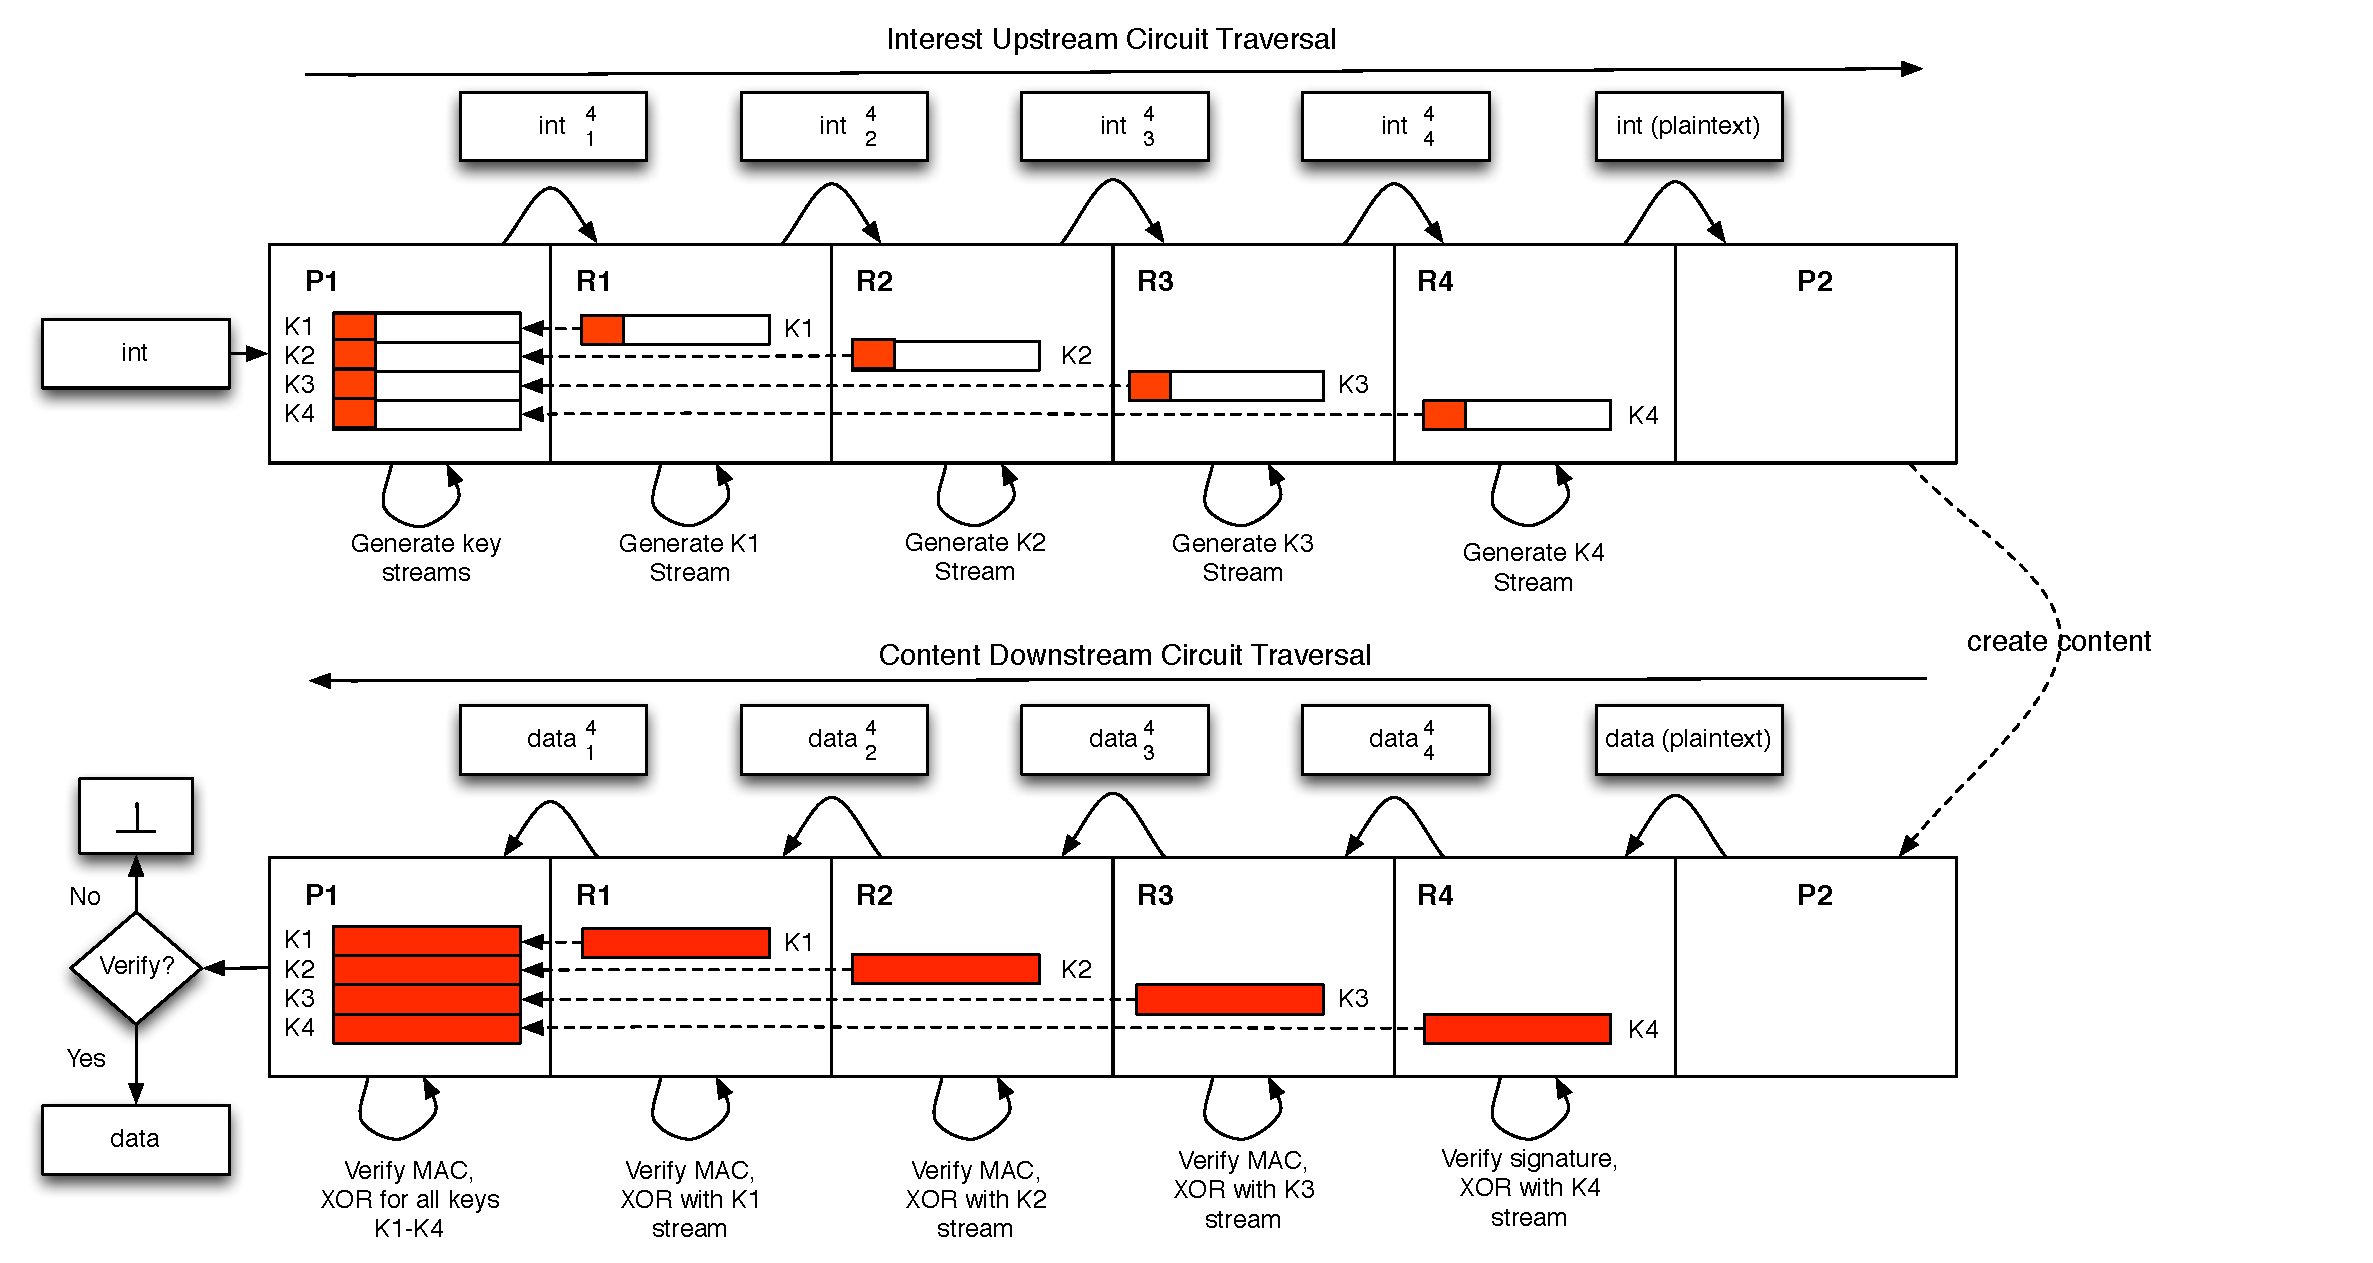
\includegraphics[scale=0.45]{./images/ctr_split.pdf}
\end{center}
\caption{Visual depiction of keystream precomputation during upstream interest traversal and the resulting half of AES-CTR that must be computed for the resulting content flowing downstream. We again emphasize that keystream ``pumping'' for AES-CTR can be done for interests as well.}
\label{fig:circuit}
\end{figure}

\section{Correctness and Security Analysis}
In order to assess the security of {\sf AND\=aNA-v2} it is important to first define an adversarial model and corresponding definition of security. To this end, we define an adversarial model for {\sf AND\=aNA-v2} that has the same capabilities as presented in \cite{andana}:
\begin{itemize}
	\item Deploy compromised routers
	\item Compromise existing routers
	\item Control content producers
	\item Deploy compromised caches
	\item Observe and replay traffic
\end{itemize}
Furthermore, any of these actions or capabiltiies can be carried out adaptively (i.e., in response to status updates from the network or based on the adversary's observations). We also note that the time required to carry out an attack is non-negligibly larger than the average RTT for an interest-content exchange in order to make this model realistic. 

We also make use of the same notions of producer and consumer anonymity and unlinkability to define the security of this scheme. Before reintroducing these definitions, we first establish the relevant notation. An adversary $\mathcal{A}$ is defined as a 4-tuple $(\mathsf{P}_{\mathcal{A}}, \mathsf{C}_{\mathcal{A}}, \mathsf{R}_{\mathcal{A}}, \mathsf{IF}_{\mathcal{A}})$, where each individual component denotes the set of producers, consumers, routers, and interfaces compromised by $\mathcal{A}$, respectively. Following \cite{andana}, a router $r$ is deemed compromised (i.e., $r \in \mathcal{R}_{\mathcal{A}}$) if all of its interfaces belong to $\mathsf{IF}_{\mathcal{A}}$. Similarly, if $\mathcal{A}$ controls a producer or consumer then they have complete (and adaptive) control over how they behave in the application session, meaning that $\mathcal{A}$ can control everything from the timing, format, and actual information of each piece of content. We also define the anonmity set with respect to an interface $\mathsf{if}_i^r$ (i.e., interface $i$ of router $r$) to be 
\begin{align*}
\mathsf{AS}_{\mathsf{if}_{i}^{r}} = \{d | \Pr[d \to_\mathsf{int} r | \mathsf{int} \to \mathsf{if}_i^r] > 0 \},
\end{align*}
and the anonymity set with respect to the adversary $\mathcal{A}$ to be
\begin{align*}
\mathsf{AS}_{\mathcal{A}}^{\mathsf{int}} = \bigcap_{\mathsf{path}^{\mathsf{int}} \cap \mathsf{IF}_{\mathcal{A}}} \mathsf{AS}_{\mathsf{if}_{i}^{r}},
\end{align*}
where $\mathsf{path}^{\mathsf{int}}$ is the set of interfaces along which the interest $\mathsf{int}$ traversed in the circuit from the consumer to the producer. 

Finally, we denote the ``state'' of a network, or configuration, as a snapshot in time of its current activity. Accordingly, each configuration is a relation that maps parties to their actions (e.g., interest or content creation). For circuits of length $n$, let a configuration $C$ be defined as
\begin{align*}
C : \mathsf{C} \to \{(r_1,\dots,r_n,p,\overline{\mathsf{int}}_1^n)\},
\end{align*}
where the $(n + 2)$-element tuple $(r_1,\dots,r_n,p,\mathsf{int}_1^n) \in \mathsf{R}^n \times \mathsf{P} \times \{0,1\}^*$. This relation can be viewed as a map from a consumer $c \in \mathsf{C}$ to a set of routers defining the circuit from $c$ to all producers $p \in \mathsf{P}$ along which interests $\overline{\mathsf{int}}_1^n$ traverse. 

Following in the footsteps of \cite{andana}, we define the security of our design in the context of indistinguishable network configurations. Specifically, two configurations $C$ and $C'$ are said to be \emph{indistinguishable with respect to $\mathcal{A}$}, denoted $C \equiv_{\mathcal{A}} C'$, if for all such polynomial-time adversaries $\mathcal{A}$ there exists a negligible function $\epsilon$ such that 
\begin{align*}
\left|\Pr[\mathcal{A}(1^n, C) = 1] - \Pr[\mathcal{A}(1^n, C') = 1]\right| \leq \epsilon(\kappa),
\end{align*}
for the global security parameter $\kappa$.

We now define security of our design in terms of consumer and producer anonymity and unlinkability. These can be found in \cite{andana}, but we provide them here for completeness. We also provide new definitions that make sense in the context of the bidirectional session case that {\sf AND\=aNA-v2} is intended to support.
\begin{defn}
\cite{andana} For $u \in (\mathsf{C} \setminus \mathsf{C}_{\mathcal{A}})$, $u$ is said to have {\sf consumer anonymity} in configuration $C$ with respect to adversary $\mathcal{A}$ if there exists $C' \equiv_{\mathcal{A}} C$ such that $C'(u') = C(u)$ and $u' \not= u$. 
\end{defn}
\begin{defn}
\cite{andana} Given $\overline{\mathsf{int}}_1^n$ and $p \in \mathsf{P}$, $u \in \mathsf{C}$ has {\sf producer anonymity} in configuration $C$ with respect to $p$ and adversary $\mathcal{A}$ if there exists a configuration $C' \equiv_{\mathcal{A}} C$ such that $\overline{\mathsf{int}}_1^n$ is sent by a non-compromised consumer to a producer different from $p$. 
\end{defn}
\begin{defn}
Two entities $u_1$ and $u_2$, both serving as producer and consumer of content in an application session, are said to have {\sf session anonymity} in configuration $C$ with respect to adversary $\mathcal{A}$ if both $u_1$ and $u_2$ enjoy producer and consumer anonymity in $C$ with respect to $\mathcal{A}$.
\end{defn}
\begin{defn}
\cite{andana} We say that $u \in (\mathsf{C} \setminus \mathsf{C}_{\mathcal{A}})$ and $p \in \mathsf{P}$ are {\sf unlinkable} in $C$ with respect to an adversary $\mathcal{A}$ if there exists a configuration $C' \equiv_{\mathcal{A}} C$ where $u$'s interests are sent to a producer $p' \not= p$.
\end{defn}

We emphasize that the fundamental differences between the design of {\sf AND\=aNA} and {\sf AND\=aNA-v2} are that, in {\sf AND\=aNA-v2}, each adjacent router will share a private MAC key used for efficient content signature generation (and, optionally, verification) and sessions are identified by the output of $H$ (rather than encrypting and decrypting interests using expensive asymmetric procedures). Accordingly, the proofs of anonymity and privacy need to be augmented to take this into account. The remainder of the design is syntactically equivalent to that of {\sf AND\=aNA}, and so we may restate the theoreoms without proof. However, in doing so, we generalize them to circuits of length $n \geq 2$. 

\begin{thm}
Consumer $u \in (\mathsf{C} \setminus \mathsf{C}_{\mathcal{A}})$ has consumer anonymity in configuration $C$ with respect to adversary $\mathcal{A}$ if there exists $u \not= u'$ such that any of the following conditions hold:
\begin{enumerate}
	\item $u, u' \in \mathsf{AS}_{\mathcal{A}}^{C_4(u)}$
	\item There exists ARs $r_i$ and $r_i'$ such that $r_i,r_i' \notin \mathsf{R}_{\mathcal{A}}$, both $r_i$ and $r_i'$ are on the circuit traversed by $C_4(u) = \overline{\mathsf{int}}_1^n$.
\end{enumerate}
\end{thm}
\begin{proof}
See \cite{andana}.
\end{proof}

\begin{thm}
Consumer $u$ has producer anonymity in configuration $C$ with respect to producer $p \in \mathsf{P}$ and adversary $\mathcal{A}$ if there exists a pair of ARs $r_i$ and $r_i'$ such that $r_i$ and $r_i'$ (for some uncompromised entity $u \notin \mathsf{C}_{\mathcal{A}}$) are on the path traversed by $C_4(u) = \overline{\mathsf{int}}_1^n$, $C_1(u) = C_1(u')$, and $C_3(u) = p \not= C_3(u')$.
\end{thm}
\begin{proof}
See \cite{andana}.
\end{proof}

\begin{cor}
Consumer $u \in (\mathsf{C} \setminus \mathsf{C}_{\mathcal{A}})$ and producer $p \in \mathsf{P}$ are unlinkable in configuration $C$ with respect to adversary $\mathcal{A}$ if $p$ has producer anonymity with respect to $u$'s interests or $u$ has consumer anonymity and there exists a configuration $C' \equiv_{\mathcal{A}} C$ where $C'(u') = C(u)$ with $u' \not= u$ and $u'$'s interests have a destination different from $p$. 
\end{cor}

In addition to security, we must also be concerned about the correct functioning of each AR supporting a session between two parties. In this context, we (informally) define session correctness as the ability of a consumer to correctly decrypt content that is generated \emph{in response to} its original interest. That is, if a consumer issues an interest, it should be able to correctly decrypt the content that it receives. The following factors impact the correctness of the session:
\begin{enumerate}
  \item Each AR $r_1,\dots,r_n$ on the consumer-to-producer circuit should correctly recover the session identifier associated with the current session. 
  \item The session key streams should only be advanced upon the receipt of an interest corresponding to the consumer who initiated the session or content that is generated from the upstream router (potentially the producer) in the circuit.
\end{enumerate}

The first item is necessary in order for each AR to correctly decrypt interests, encrypt content, and perform content signature generation and verification. The second item is necessary so that all content can be correctly decrypted by the consumer. We claim that, given a CCA-secure public key encryption scheme, the probability that either one of these factors being violated by an adversary $\mathcal{A}$ is negligible. Let $\mathsf{ForgeSession}$ and $\mathsf{KeyJump}$ denote the events corresponding to instances where an adversary creates a ciphertext that maps to a valid session identifier for \emph{some} session currently supported by an AR (i.e., the forged session belongs to the routers session table $\mathsf{ST}$), and the event that an adversary causes the key stream for \emph{some} AR in a consumer-to-producer circuit to fall out of sync with the consumer. By the design of {\sf AND\=aNA-v2}, it should be clear that $\mathsf{KeyJump}$ occurs when $\mathsf{ForgeSession}$ occurs, since the key stream is only advanced upon receipt of an interest, but may also occur when an adversary successfully forges a MAC tag corresponding to the signature of a piece of content from the upstream router (or producer). We denote this latter event as $\mathsf{ContentMacForge}$. With the motivation in place, we now formally analyze the probabilities of these events occuring below. For notational convenience, we assume that each event only occurs as a result of some adversarial action, so we omit this relation in what follows.

\begin{lemma}
For all probabilistic polynomial-time adversaries $\mathcal{A}$, there exists some negligible function $\mathsf{negl}$ such that
\begin{align*}
\Pr[\mathsf{ForgeSession}] \leq \mathsf{negl}(\kappa).
\end{align*}
\end{lemma}
\begin{proof}
By the design of {\sf AND\=aNA-v2}, we know that session identifiers are computed as the output of a collision resistant hash function $H : \{0,1\}^* \to \{0,1\}^{m}$, where $m = \mathsf{poly}(\kappa)$ (i.e. polynomial in the global security parameter). Consequently, forging a session identifier \emph{without} the input to $H$ implies that a collision was found, thus violating collision resistance of $H$. Thus, forging a session is equally hard as finding a collision in $H$, or more formally, $\Pr[\mathsf{Collision}(H) = 1] = \Pr[\mathsf{ForgeSession}]$. By the properties of collision resistance of $H$ which states that $\Pr[\mathsf{Collision}(H) = 1] \leq \mathsf{negl}(\kappa)$ for some negligible function $\mathsf{negl}$, it follows that $\Pr[\mathsf{ForgeSession}] \leq \mathsf{negl}(\kappa)$. 

% TODO: asusme that some session is forged... session identifiers are created from hashing the session ID as per the above design, so a forgery implies a collision in the hash function. If we assume a CRH hash, then forgery implies contradiction, and we're done.
\end{proof}

\begin{lemma}
For all probabilistic polynomial-time adversaries $\mathcal{A}$, there exists some negligible function $\mathsf{negl}$ such that
\begin{align*}
\Pr[\mathsf{ContentMacForge}] \leq \mathsf{negl}(\kappa).
\end{align*}
\end{lemma}
\begin{proof}
By the design of {\sf AND\=aNA-v2}, the MAC scheme $\Pi$ used for content symmetric content signature generation and verification is defined as $\Pi = (\mathsf{Gen}, \mathsf{Mac}, \mathsf{Ver})$, where $\mathsf{Gen}$ generates the secret key $k$ used in the scheme, $\mathsf{Mac}_k(m)$ outputs the MAC tag $t := F_k(m)$ for some pseudorandom function $F$, and $\mathsf{Ver}_k(m, t)$ outputs $1$ if $t = \mathsf{Mac}_k(m)$ and $0$ otherwise. This is known and proven to be a secure MAC scheme [does this warrant citation?], meaning that for all probabilistic polynomial-time adversaries $\mathcal{A}$ there exists a negligible function $\mathsf{negl}$ such that $\Pr[\mathsf{MacForce}_{\mathcal{A},\Pi}(1^{\kappa}) = 1] \leq \mathsf{negl}(\kappa)$, and since $\mathsf{ContentMacForce}$ occurs exactly when the even $\mathsf{MacForce}$ occurs, we have that $\Pr[\mathsf{ContentMacForge}] \leq \mathsf{negl}(\kappa)$.

% TODO: assume secure MAC scheme based on PRF is used, a forgery in the MAC scheme therefore relies on the PRFness of SipHash... If this holds, then ContentMacForge is negligible.
\end{proof}

\begin{lemma}
For all probabilistic polynomial-time adversaries $\mathcal{A}$, there exists some negligible function $\mathsf{negl}$ such that
\begin{align*}
\Pr[\mathsf{KeyJump}] \leq \mathsf{negl}(\kappa).
\end{align*}
\end{lemma}
\begin{proof}
By the design of {\sf AND\=aNA-v2}, it follows that $\Pr[\mathsf{KeyJump}] = \Pr[\mathsf{ForgeSession}] + \Pr[\mathsf{ContentMacForce}]$, and since the sum of two negligible functions is also negligible, it follows that there exists some negligible function $\mathsf{negl}$ such that $\Pr[\mathsf{KeyJump}] \leq \mathsf{negl}(\kappa)$.
\end{proof}

\begin{thm}
Session correctness of {\sf AND\=aNA-v2} is only violated with negligible probability.
\end{thm}
\begin{proof}
This follows immediately from Lemmas 1, 2, and 3 and the fact that the sum of two negligible functions is also negligible.\footnote{This sum comes from the fact that the probability of the ``failure'' events occurring must be taken into account in both directions of the session.} 
\end{proof}

\section{Preliminary Performance Evaluation}
In order to justfiy {\sf AND\=aNA-v2} as an alternative to existing solutions for low-latency, bidirectional traffic over NDN, we must first establish a baseline of performance metrics against which we can compare our design. Since the original version of {\sf AND\=aNA} targeted circuits of length $2$ (i.e., with two ARs), we focus on the same length circuits in these experiments. We note that there is nothing restricting us from lifting this constraint in future experiments. In order to adequately determine a baseline of performance metrics, we instantiated two parties (both acting as a data producer and consumer) interacting by requesting moderately-sized content in short, frequent intervals. In order ensure that such content is never satisfied by the cache of an intervening AR, which is a reasonable assumption for real-time voice and video applications that always want fresh content instead of stale cached content, each piece of content is requested from an anonymized namespace and indexed by a sequence number. For example, if the two parties $P_1$ and $P_2$ are communicating and $P_1$ wants to request the latest content from $P_2$, it will issue an (encrypted)interest to {\tt ccnx:/$P_2$/$S$}, where $S$ is the sequence number that is incremeneted as soon as the interest is issued. This ensures that such interests are never satisfied by the content in an AR cache throughout the duration of the session. 

With this type of traffic generation application, we then tested its performance under the following scenarios:
\begin{enumerate}
  \item $P_1$ and $P_2$ are connected point-to-point (i.e., no hops).
  \item $P_1$ and $P_2$ are connected through two ``insecure'' ARs that perform no interest or content encryption (i.e., each AR just serves as an application-level proxy to forward interests and content along through the circuit).
  \item $P_1$ and $P_2$ are connected through two ``secure'' ARs that perform interest and content encryption as per the {\sf AND\=aNA} design.
\end{enumerate}
Table \ref{tab:baseline} shows the performance results from such scenarios 1, 2, and 3, in which performance is characterized as the end-user latency between issuing an interest and receiving the intended content. In this case, we refer to the performance in terms of latency, where $L_i$ denote the average latency and $\sigma_i$ denote its standard deviation for party $i$ ($i \in \{1,2\}$). All experiments were collected using the following methdology:
\begin{itemize}
  \item Each party generates 1000 traffic according to an uniform distribution with $pmf = 1/100$. 
  \item Each party responds to all interests with a random blob of 150 bytes. \footnote{This value was chosen to match the average size of a Skype video call packet. Are experiments with different size pieces of content warranted for this proof of concept?}
\end{itemize}

\begin{table}
\centering
\caption{Baseline performance metrics gathered from the three scenarios discussed in the text.}
\label{tab:baseline}
  \begin{tabular}{|c || c c | c c|} \hline
  Scenario & $L_1$ & $\sigma_1$ & $L_2$ & $\sigma_2$ \\ \hline
  1 & $0.00735$ & $0.00798$ & $0.00340$ & $0.00053$ \\
  2 & $0.01905$ & $0.13791$ & $0.02248$ & $0.13923$ \\
  3 & $0.01321$ & $0.00257$ & $0.01359$ & $0.00567$ \\ \hline
  \end{tabular}
\end{table}

According to the preliminary experimental evaluation, it appears as though low-latency, bidirectional communication is realtively feasible with the current {\sf AND\=aNA} design. However, we would like to do better. 


% To that end, we first formally capture the performance of the {\sf AND\=aNA} (symmetric variant) and {\sf AND\=aNA-v2} designs to enable quantitative comparison using the concrete cryptographic primitives discussed in the previous following section. First, let $T_1^{\mathsf{S}}$ and $T_2^{\mathsf{A}}$ be the expected total time required to retrieve one piece of content in the symmetric {\sf AND\=aNA} and asymmetric {\sf AND\=aNA-v2} designs, respectively. Assume that a circuit consists of $n$ ARs, all encrypted interests consist of a single 128-bit block, and all respective content packets consist of $b$ 128-bit blocks. Finally, let $T_{\mathsf{AES}}$, $T_{\mathsf{HMAC}}$, $T_{\mathsf{XOR}}$, $T_{\mathsf{RSA}}$, $T_{\mathsf{MAC}}$, and $T_{\mathsf{HASH}}$ denote the time required to perform AES, HMAC, XOR, RSA, MAC, and an arbitrary hash function computation, respectively. Note that we separate the time required to encrypt a single block of plaintext with AES from the corresponding MAC scheme (i.e., HMAC or GHASH) for notational convenience. We also introduce the additional quantities $H_1 = \sum_{i=0}^{n-1}i$ and $H_b = \sum_{i=0}^{n-1}(b + i)$, which will be used to count the blocks of ciphertext that are accumulated as interests and content flow upstream and downstream. We now present the expressions for $T_1^{\mathsf{S}}$ and $T_2^{\mathsf{A}}$ as follows:

% %%% In both, Hash of content increases by 1 since each ciphertext includes a new single block tag, encryption is just remasking the same set of bits over and over again, so the ciphertext never grows in size this way (i.e. ciphertext from upstream serves as plaintext for the downstream)
% \begin{align*}
% T_1^{\mathsf{S}} & = \underbrace{2n(T_{\mathsf{AES}} + T_{\mathsf{HMAC}}) }_{\text{interests}} + \underbrace{2nb(T_{\mathsf{AES}} + T_{\mathsf{HMAC}}) }_{\text{content encryption}} + \underbrace{2T_{\mathsf{HASH}}\left(nb + \frac{n(n+1)}{2}\right) + 2nT_{\mathsf{RSA}}}_{\text{sign/verify}}  %nb cost for hash at each AR and signer (ciphertext doesn't accumulate)
% \end{align*}

% \begin{align*}
% T_2^{\mathsf{A}} & = \underbrace{2n(T_{\mathsf{HASH}} + T_{\mathsf{AES}} + T_{\mathsf{XOR}}) }_{\text{interest encr/decr}} + \underbrace{2n(b+1)T_{\mathsf{XOR}} }_{\text{content encr/decr}} + \underbrace{2T_{\mathsf{HASH}}\left(nb + \frac{n(n+1)}{2}\right) + 2nT_{\mathsf{MAC}}}_{\text{sign/verify}}
% \end{align*}

% It is important to emphasize that we are comparing the symmetric variant of {\sf AND\=aNA} with the asymmetric variant of {\sf AND\=aNA-v2}. As stated in \cite{andana}, the symmetric variant does not enjoy consumer and producer unlinkability since session identifiers are sent in cleartext. However, for the sake of comparing performance, we opted to compare the \emph{best} version of {\sf AND\=aNA} with the \emph{worst} variant of {\sf AND\=aNA-v2}. Accordingly, comparing the performance of these two seemingly uncompatible designs will serve to intensify the improvement of the {\sf AND\=aNA-v2} design both in terms of performance (for this particular use case) and security/anonymity. 
% As one can see, $T_1^{\mathsf{S}}$ and $T_2^{\mathsf{A}}$ are quite different. While content signature generation seemingly consumes the majority of the computation in the {\sf AND\=aNA} design, the {\sf AND\=aNA-v2} design enjoys highly efficient content signature generation by using symmetric MACs. Since adjacent ARs in the circuit share a common MAC key that is established during the circuit and session establishment protocol, a MAC can effectively remove the need for an expensive hash computation (on possibly large messages) and subsequent signature. Furthermore, there are no asmmetric cryptographic operations needed for this new design, which intuitively means that it will achieve better performance. Of course, we require empirical evidence to support this claim, and the implementation and evaluation of {\sf AND\=aNA-v2} will provide exactly that information.

%%%%%%%%%%%%%%%%%%%%%
%%% END MAIN CONTENT
%%%%%%%%%%%%%%%%%%%%%

%%% BIBLIOGRAPHY
\begin{thebibliography}{[MT1]}

\bibitem{voccn} V. Jacobson, D. K. Smetters, N. H. Briggs, M. F. Plass, P. Stewart, J. D. Thornton, and R. L. Braynard. VoCCN: Voice-Over Content-Centric Networks. \emph{In Proceedings of the 2009 Workshop on Re-Architecting the Internet (ReArch '09), ACM, New York, NY, USA} (2009), 1-6. 

\bibitem{andana} S. DiBenedetto, P. Gasti, G. Tsudik, and E. Unzun. {\sf AND\=aNA}: Anonymous named data networking application. \emph{In NDSS '12} (2012).

\bibitem{tor} R. Dingledine, N. Mathewsonn, and P. Syverson. Tor: The Second-Generation Onion Router. \emph{In The 13th USENIX Security Symposium} (2004).

\bibitem{nist-sha3} S. Chang, R. Perlner, W. E. Burr, M. S. Turan, J. M. Kelsey, S. Paul, L. E. Bassham. Third-Round Report of the SHA-3 Cryptographic Hash Algorithm Competition. \emph{National Institute of Standards and Technology (NIST) NISTIR 7896}.

\bibitem{siphash} J. Aumasson and D. J. Bernstein. SipHash: A Fast Short-Input PRF. \emph{Progress in Cryptology - INDOCRYPT 2012, Springer Berlin Heidelberg} (2012), 489-508.

\bibitem{aesgcm-intel} S. Gueron. AES-GCM for Efficient Authenticated Encryption - Ending the Reign of HMAC-SHA-1? \emph{Workshop on Real-World Cryptography, Stanford University, CA} (2013).

\bibitem{attacking-unlinkability} M. Franz, B. Meyer, and A. Pashalidis. Attacking Unlinkability: The Importance of Context. \emph{Privacy Enhancing Technologies. Springer Berlin Heidelberg} (2007).

\bibitem{linkability-attacks} S. Schiffner and S. ClauB. Using Linkability Information to Attack Mix-Based Anonymity Services. \emph{Privacy Enhancing Technologies. Springer Berlin Heidelberg} (2009).

\bibitem{tor-traffic-analysis} S. J. Murdoch and G. Danezis. Low-Cost Traffic Analysis of Tor. \emph{2005 IEEE Symposium on Security and Privacy} (2005).

\bibitem{keccak-files} The Keccak sponge function family. Software and other files. Available online at \url{http://keccak.noekeon.org/files.html}. Last accessed 11/18/13.

\bibitem{ndn-tech-report} Lixia Zhang, Deborah Estrin, Jeffrey Burke, Van Jacobson, Jim Thornton, Diana K. Smetters, Beichuan Zhang, Gene Tsudik, kc claffy, Dmitri Krioukov, Dan Massey, Christos Papadopoulos, Tarek Abdelzaher, Lan Wang, Patrick Crowley, and Edmund Yeh. Named Data Networking (NDN) Project. \emph{Technical Report NDN-0001, Xerox Palo Alto Research Center - PARC} (2010).

\bibitem{piggyback} Mishari Almishari, Paolo Gasti, Naveen Nathan, and Gene Tsudik. Optimizing Bi-Directional Low-Latency Communication in Named Data Networking. \emph{arXiv preprint} arXiv:1207.7085 (2012).

% \bibitem{keccak-sw} The Keccak sponge function family. Software performance figures. Available online at \url{http://keccak.noekeon.org/sw_performance.html}. Last accessed 11/18/13.

\end{thebibliography}

\end{document}
